\documentclass[12pt,a4paper,oneside]{book}

%include the configuration file for layout
%Have a look in this file it has some useful commands defined
\usepackage{setspace}
\usepackage{geometry}
\usepackage[toc,page]{appendix}
\usepackage{lipsum}
\usepackage[export]{adjustbox}
\usepackage[T1]{fontenc}
\usepackage{textcomp}
\usepackage{epsfig,graphics}
\usepackage{graphicx}
\usepackage{titlesec}
\usepackage[parfill]{parskip}
\usepackage{hyperref}
\usepackage{url}
\usepackage{pdflscape} % Provides the landscape environment
\usepackage{pgfplots, pgfplotstable}
\usepgfplotslibrary{statistics}
\usepackage{cleveref}
\usepackage{textcomp}
\usepackage{multicol}
\usepackage{pgfgantt}

% Tables
% \usepackage[utf8]{inputenc}
% \setlength{\arrayrulewidth}{1mm}
% \setlength{\tabcolsep}{18pt}
% \renewcommand{\arraystretch}{1.5}

% Images and fixed position stuff
% \usepackage{subfig}
\usepackage{float}
\usepackage{subcaption}

\usepackage{pgfgantt}
\usepackage{pdflscape} % Provides the landscape environment
\usepackage{subcaption}


% Code portions stuff
\usepackage{listings}
\usepackage{color}

\definecolor{dkgreen}{rgb}{0,0.6,0}
\definecolor{gray}{rgb}{0.5,0.5,0.5}
\definecolor{mauve}{rgb}{0.58,0,0.82}

\lstset{frame=tb,
  language=Python,
  aboveskip=3mm,
  belowskip=3mm,
  showstringspaces=false,
  columns=flexible,
  basicstyle={\small\ttfamily},
  numbers=none,
  numberstyle=\tiny\color{gray},
  keywordstyle=\color{blue},
  commentstyle=\color{dkgreen},
  stringstyle=\color{mauve},
  breaklines=true,
  breakatwhitespace=true,
  tabsize=3
}

%%%%%%%%%%%%%%%%%%%%%%%%%%%%%%%%%%%%%%%%%%%%%%%%%%%%%%%%%%%%%%%%%%%%%%%%%%%%%%
% Details of your dissertation
%%%%%%%%%%%%%%%%%%%%%%%%%%%%%%%%%%%%%%%%%%%%%%%%%%%%%%%%%%%%%%%%%%%%%%%%%%%%%%
\newcommand{\projectTitle}{Human Aware Robot Navigation}
\newcommand{\fullname}{Ilyass Taouil}
\newcommand{\degreeTitle}{BSc Artificial Intelligence}
\newcommand{\session}{2017/2018}
\newcommand{\credits}{60 credits}		% i.e. "60 credits"" or "40 credits""

%%%%%%%%%%%%%%%%%%%%%%%%%%%%%%%%%%%%%%%%%%%%%%%%%%%%%%%%%%%%%%%%%%%%%%%%%%%%%%
% Change the geometry of the page to have a 25 mm binding edge
%%%%%%%%%%%%%%%%%%%%%%%%%%%%%%%%%%%%%%%%%%%%%%%%%%%%%%%%%%%%%%%%%%%%%%%%%%%%%%
 \geometry{
 a4paper,
 total={210mm,297mm},
 left=25mm,
 right=25mm,
 top=25mm,
 bottom=20mm,
 }
 
%%%%%%%%%%%%%%%%%%%%%%%%%%%%%%%%%%%%%%%%%%%%%%%%%%%%%%%%%%%%%%%%%%%%%%%%%%%%%%
% Commands to set the line spacing
%%%%%%%%%%%%%%%%%%%%%%%%%%%%%%%%%%%%%%%%%%%%%%%%%%%%%%%%%%%%%%%%%%%%%%%%%%%%%%
 %\singlespacing
 \onehalfspacing
 %\doublespacing
 
%%%%%%%%%%%%%%%%%%%%%%%%%%%%%%%%%%%%%%%%%%%%%%%%%%%%%%%%%%%%%%%%%%%%%%%%%%%%%%
% Spacing for the chapter header
%%%%%%%%%%%%%%%%%%%%%%%%%%%%%%%%%%%%%%%%%%%%%%%%%%%%%%%%%%%%%%%%%%%%%%%%%%%%%%
 \titleformat{\chapter}[display]
    {\normalfont\Huge\bfseries}{\vspace*{-1\baselineskip}\chaptertitlename\ \thechapter}{15pt}{\huge}
\titlespacing*{\chapter}{0pt}{0pt}{15pt}

\renewcommand\bibname{References}

%%%%%%%%%%%%%%%%%%%%%%%%%%%%%%%%%%%%%%%%%%%%%%%%%%%%%%%%%%%%%%%%%%%%%%%%%%%%%%
% Some shortcuts that maybe useful
%%%%%%%%%%%%%%%%%%%%%%%%%%%%%%%%%%%%%%%%%%%%%%%%%%%%%%%%%%%%%%%%%%%%%%%%%%%%%%
\DeclareTextCommandDefault{\textcopyright}{\textcircled{c}}
 
%%%%%%%%%%%%%%%%%%%%%%%%%%%%%%%%%%%%%%%%%%%%%%%%%%%%%%%%%%%%%%%%%%%%%%%%%%%%%%
% Bibliography style: choose one and make sure you have the relevant .bst file
%%%%%%%%%%%%%%%%%%%%%%%%%%%%%%%%%%%%%%%%%%%%%%%%%%%%%%%%%%%%%%%%%%%%%%%%%%%%%%
\bibliographystyle{abbrv}


%%%%%%%%%%%%%%%%%%%%%%%%%%%%%%%%%%%%%%%%%%%%%%%%%%%%%%%%%%%%%%%%%%%%%%%%%%%%%%
% Layout for the front cover !!!!! YOU SHOULD NOT HAVE TO CHANGE THIS!!!!!
%%%%%%%%%%%%%%%%%%%%%%%%%%%%%%%%%%%%%%%%%%%%%%%%%%%%%%%%%%%%%%%%%%%%%%%%%%%%%%
 
\newcommand{\frontcover}{
% The title page:
\begin{titlepage}
\newgeometry{left=25mm,right=25mm,top=45mm,bottom=0.1cm}

\begin{minipage}[t]{7cm}
\noindent\textbf{\Large{School of Computing}}\\
{\fontfamily{ptm}\selectfont 
\uppercase{faculty of engineering}
}
\end{minipage}
\hfill
\begin{minipage}[t]{7cm}
\vspace*{-25pt}

\includegraphics[scale=0.2,right]{logo_black.png}
\vspace*{-1pt}
\end{minipage}

\noindent\makebox[\linewidth]{\rule{\paperwidth}{0.4pt}}

\centering
\vspace*{37mm}
\textbf{\Large\projectTitle}\\
\vspace*{10mm}
\textbf{\large\fullname}\\
\vspace*{10mm}
\textbf{Submitted in accordance with the requirements for the degree of}\\
\textbf{\degreeTitle}\\
\vspace*{10mm}
\session\\
\vspace*{10mm}
\credits\\
\restoregeometry
\end{titlepage}
}

%%%%%%%%%%%%%%%%%%%%%%%%%%%%%%%%%%%%%%%%%%%%%%%%%%%%%%%%%%%%%%%%%%%%%%%%%%%%%%
% Define a new environment for the dissertation summary
%%%%%%%%%%%%%%%%%%%%%%%%%%%%%%%%%%%%%%%%%%%%%%%%%%%%%%%%%%%%%%%%%%%%%%%%%%%%%%
\newenvironment{dissertationsummary}
 	{\cleardoublepage \null 
 		\begin{center}%
			\textbf{Summary}
		\end{center}}%
	{\vfill \null }

\begin{document}
  % The prelude is everything up to the start of chapter 1. Including the
  % cover page, deliverable page, summary, acknowledgements and table of
  % contents.
  \pagenumbering{roman}
\frontcover

\clearpage
\noindent The candidate confirms that the following have been submitted.\\
<As an example>
\begin{table}[ht!]
\begin{tabular}{|p{0.3\textwidth}|p{0.3\textwidth}|p{0.3\textwidth}|}
\hline 
Items & Format & Recipient(s) and Date \\ 
\hline 
Beliverable 1, 2, 3 & Report & SSO (DD/MM/YY) \\ 
\hline 
Participant consent forms & Signed forms in envelop & SSO (DD/MM/YY) \\ 
\hline 
Deliverable 4 & Software codes or URL & Supervisor, Assessor (DD/MM/YY) \\ 
\hline 
Deliverable 5 & User manuals & Client, Supervisor (DD/MM/YY) \\ 
\hline 
\end{tabular} 
\end{table}

\noindent Type of project: \rule{100mm}{1pt}
\vspace{\fill}\\
\noindent The candidate confirms that the work submitted is their own and the appropriate credit has been given where reference has been made to the work of others.
\vspace{\fill}\\
\noindent I understand that failure to attribute material which is obtained from another source may be considered as plagiarism.
\vspace{\fill}\\
\flushright(Signature of Student) \rule{50mm}{1pt}
\flushleft
\vspace{\fill}
\textcopyright~\session~The University of Leeds and~\fullname
% Summary

\begin{dissertationsummary}
Rudimentary robots have been part of our lives since the early stage of the industrial revolution. We interact with servicing systems almost every day, such as TV's, smartphones and self-checkout systems. This is an unstoppable trend and in the future advanced robotic systems will become more present in human environments in a variety of areas, including assistance, rescue and logistics. Moreover, interactions between humans are defined by a set of precise protocols, in fact, we would not jump in front of a queue or invade someone else's space in a common area without asking permission first. For robots to integrate they will have to comply to some ethical, moral and social rules that govern our way of being humans. The aim of this project is to contribute to the human-robot interaction domain, by developing an open-source ROS package able to estimate people's 3D position in the environment. High level of confidence and robustness were reached using deep-learning techniques to detect people in the RGB frame. RGB-D sensory data were also used to compute detections' distances with the relative 3D position in the map, using several algorithms and techniques.

\end{dissertationsummary}

\clearpage
\centering\textbf{Acknowledgements}
\flushleft
"He who does not thank people, does not thank God" (Prophet Muhammad).

I therefore would like to thank my supervisor, Dr. Matteo Leonetti, for providing help and guidance throughout the project, freedom during the development and research stages and the possibility to use an expensive piece of technology like TIAGO.

I would also like to thank the project's assessor, Dr. Mehmet Dogar, for his useful feedback and for taking time in answering the many questions I had for him.

% The contents
\tableofcontents

% The list of figures and tables Uncomments the 3 following lines
%to see a list of tables and list of figures.
%\clearpage
%\listoffigures
%\listoftables

\pagenumbering{arabic}

  % This is to reset the counter of the page to number 1 again since the table
  % of contents takes the first page for some reason. This is to ensure that
  % main content is going to be started from page 1.
  \setcounter{page}{1}

  % Chapters to be included
  \chapter{Introduction}
\label{chapter1}

\section{Context}

Rudimentary robots have been part of our lives since the early beginning of the industrial revolution. 

Nowadays we interact with servicing robots almost every day, starting from the toaster in the morning, TV and smartphones for personal entertainment to automated security checking at the airports we travel through. 

This is an unstoppable trend and in the near future robots will increasingly become more and more present in human environments in a variety of areas like assistance, grunt work, military, logistics and security.

Humans' interactions are defined by a set of precise protocols, in fact none us would carelessly jump in front of a queue or invade someone else's space in a common environment without asking permission.

Robots to be able to integrate in such an environment, and more importantly for humans to accept such an integration, will have to comply to some ethical, moral and social rules that govern our way of being humans.

In this project, the aim is to offer a starting point for such human-robot interaction, which is identifying people present in the surrounding with a certain level of confidence and robustness using several techniques and algorithms, with the final goal of creating an open-source tool to the Robotics community to tackle human aware navigation tasks.

From the intermediate report submitted at the beginning of the project some changes have occurred in the scope and planning of the project, these are outlined in appendix F. Finally, in appendix C access to the project repository, documentation and ROS package link can be found.

\section{Project Aim}

The aim of the project is to explore key-topics and main-ideas for human-aware navigation with focus on the perception side of things with the final goal of developing an open-source ROS package software product able to estimate human position in a dynamic and non-sparse environment through and ensemble approach of various algorithms and techniques, in order to facilitate human aware robot navigation.

Moreover, being this an open-source project offering interfaces for integration with other modules, modularity and ease of integration need to be features of this project.

\section{Problem Domain}

The main problems to be tackled are three, which consist in detecting the presence of people in the RGB image, get the human-robot distance and obtain the real pose (in terms of x, y and z) of the person or people in the map. 

All of these subtasks have challenges to them. In fact, the person detection module needs to be computationally efficient to be able to run real-time detections while being embedded in power constrained devices and keeping down the number of false positives and false negatives in the detection process.

The human-robot distance estimation needs to handle noise coming from the real world (lighting conditions, clutter and obstruction) while still being reliable as the real pose conversion heavily relies on a good depth estimation. 

Moreover, multiple sensors will be used for the development of the project, which on one side offers a more robust estimations process as the different sensors can complement the weaknesses of one another, however this increases the level of complexity in the integration and the possible accessibility to the ROS package, although the sensors used should be available on all standard robotics systems.

\section{Project Objectives}

The following objectives for the project are defined:

\begin{enumerate}
  \item Obtain a level of proficiency in using the ROS\footnote{Robot Operating
System} platform and its tools, including RVIZ, custom messages and packaging using CMAKE.
	\item Obtain a level of proficiency in using Robotics sensors such as RGB-D and laser-scans and in integrating them.
  \item Explore available person detection computer vision algorithms and the state-of-the-art techniques for the task.
  \item Explore available distance estimation techniques using RGB-D sensors and plain RGB data.
\end{enumerate}

\section{Project Deliverables}

The following deliverables are to be expected:

\begin{enumerate}
  \item Develop a human detection module using the robot's built-in RGB sensor.
  \item Develop a human-robot depth module to estimate the distance between the robot and the detection/s using the robot's built-in RGB-D sensor or other computer vision techniques.
  \item Integrate a leg detector algorithm for a more robust pose estimation outside of the RGB-D range.
  \item Create visual markers on RVIZ to show people's position in the map.
  \item Release the package ROS.
\end{enumerate}
  \chapter{Background Research}
\label{chapter2}

\section{Robot Operating System (ROS)}

The Robot Operating System or ROS, is a flexible framework for writing robot software. It offers libraries aiming at simplifying common robotics tasks \cite{website:aboutROS}, which otherwise would be too complex and daunting to achieve in such a broad field.

ROS is a collaborative and open-source project empowering the expertise of some of the best robotics institutions, laboratories and individuals around the globe \cite{website:aboutROS}, making ROS a well rounded framework for all types of robotics challenges. 

ROS comes in many versions. This project will make extensive use of the ROS Indigo Igloo version which targets the Ubuntu 14.04 (LTS) release.

\section{Gazebo}

Gazebo is a 3D simulator engine able to render accurately and efficiently complex indoor and outdoor environments \cite{website:Gazebo}, thereby speeding up the development process by being able to test robotics algorithms and modules via its wide and rich library of robot models and environment \cite{website:Gazebo}, without the need of particular robotics hardware.

For this project Gazebo's TIAGo extension by PAL ROBOTICS was used.

\begin{figure}[!htbp]
\begin{center}
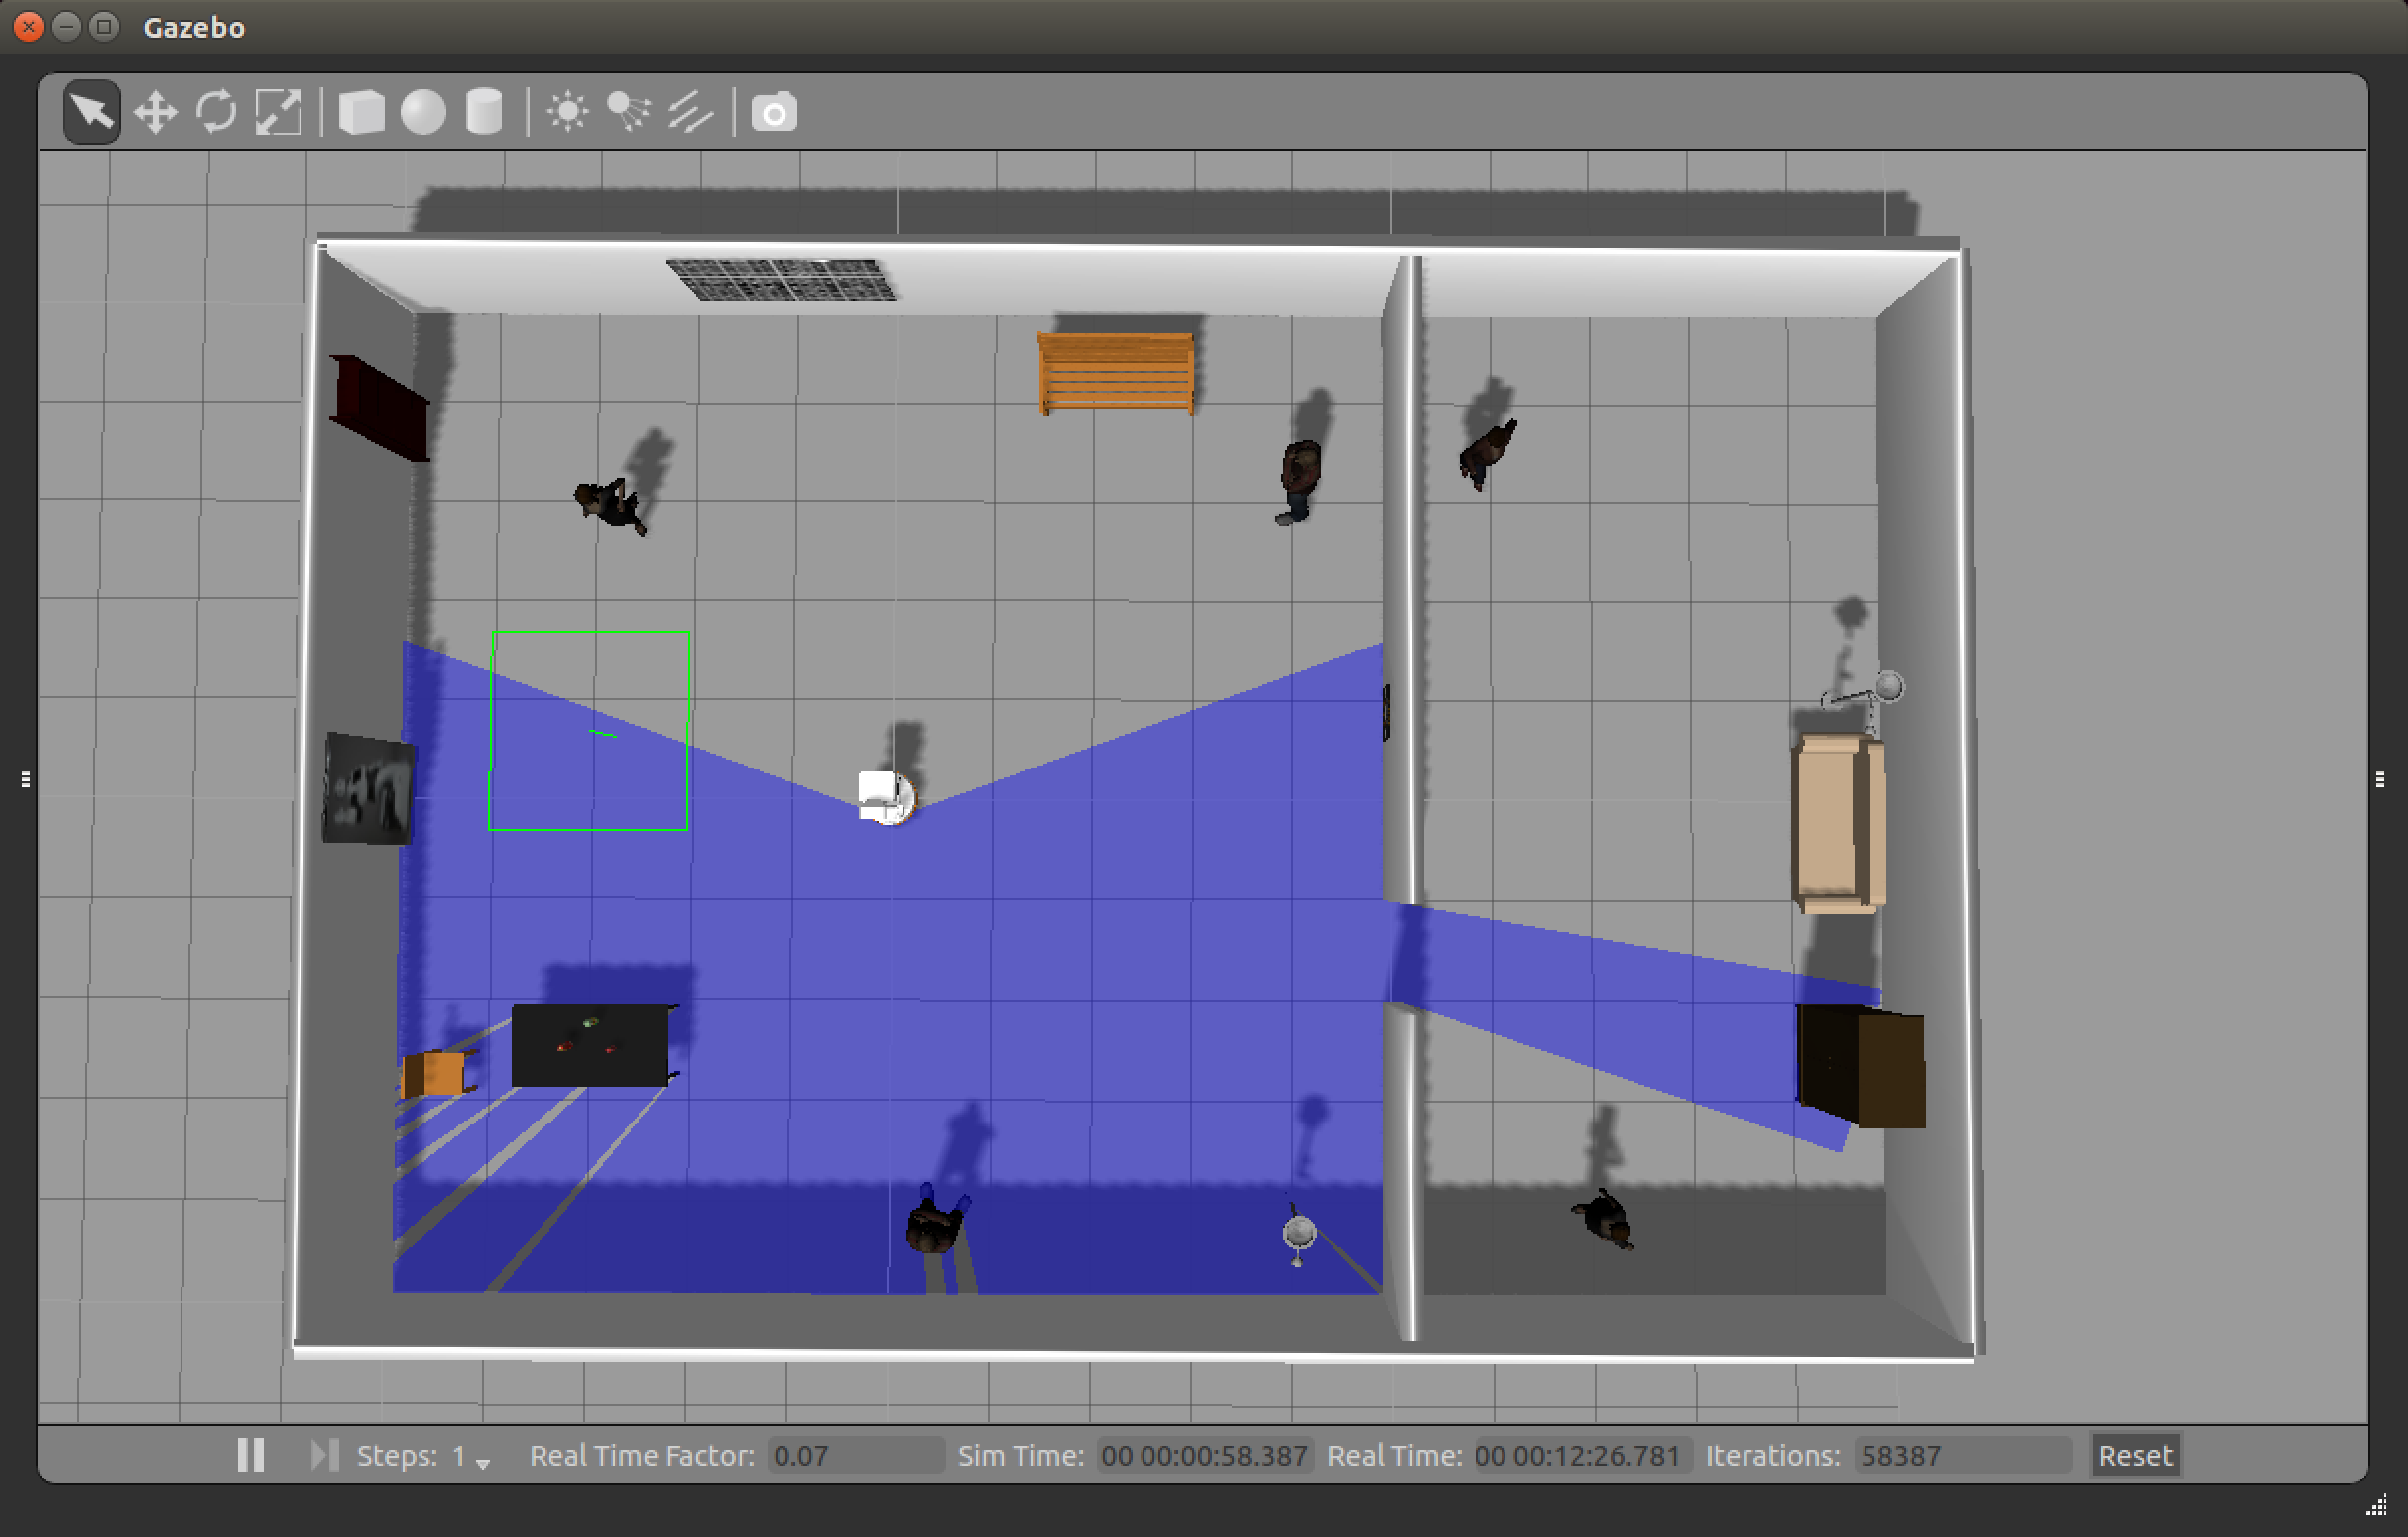
\includegraphics[width=\linewidth]{images/gazebo_screenshot1.png}
\end{center}
\caption{Gazebo Simulator (Office Environment)}
\label{fig:gazebo_screenshot1}
\end{figure}

\begin{figure}[!htbp]
\begin{center}
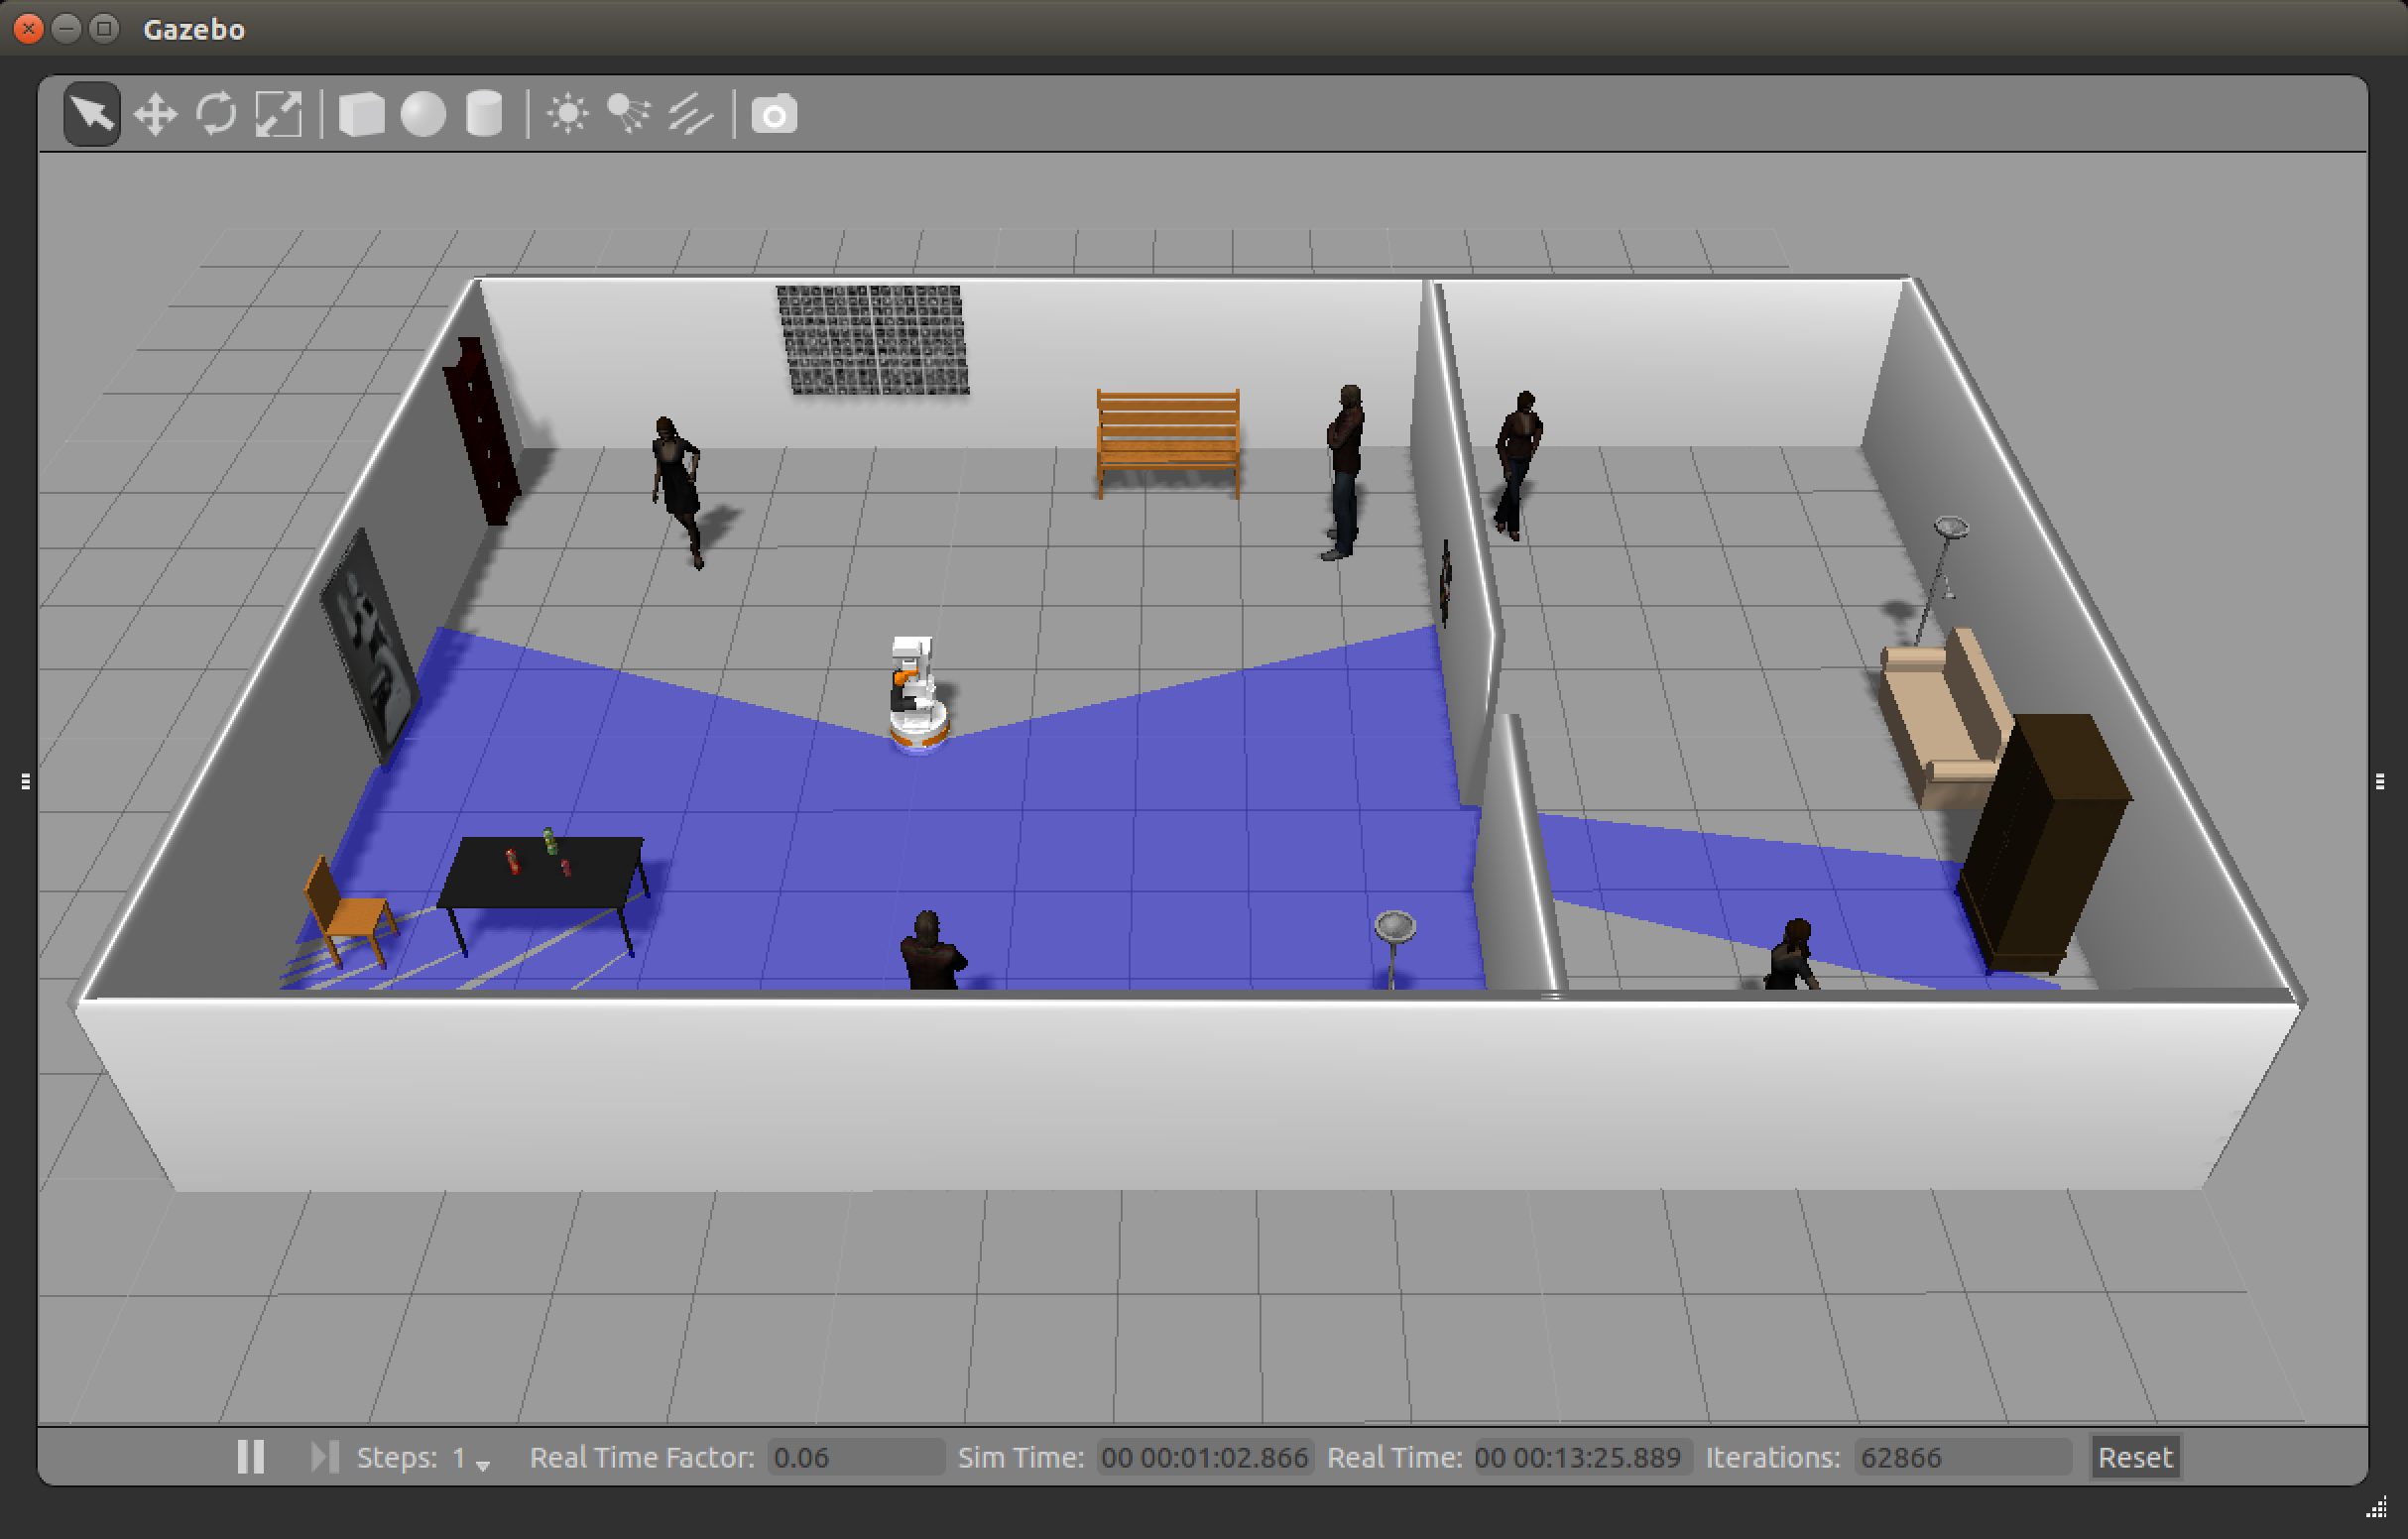
\includegraphics[width=\linewidth]{images/gazebo_screenshot2.png}
\end{center}
\caption{Gazebo Simulator (Office Environment)}
\label{fig:gazebo_screenshot2}
\end{figure}

\section{RVIZ}

RVIZ is a 3D visualisation tool that provides information about what the robot is seeing, thinking and doing. Developing robotics application is by itself a daunting task, but without exactly knowing what the robot thinks is going on in the real world it rises the level of complexity, as trying to debug only via numerical data is rather complicated especially at higher number of dimensions which is common in the robotics field \cite{website:RVIZ}. 

Other important features that RVIZ offers via its modules are point cloud visualisation, laser-scan readings, coordinate frames as well as topological maps, obstacles data and current path visualisation when using the ROS navigation stack making of RVIZ a powerful tool for this project and generally for the development of robot capabilities and research \cite{website:RVIZ}.

\begin{figure}[!htbp]
\begin{center}
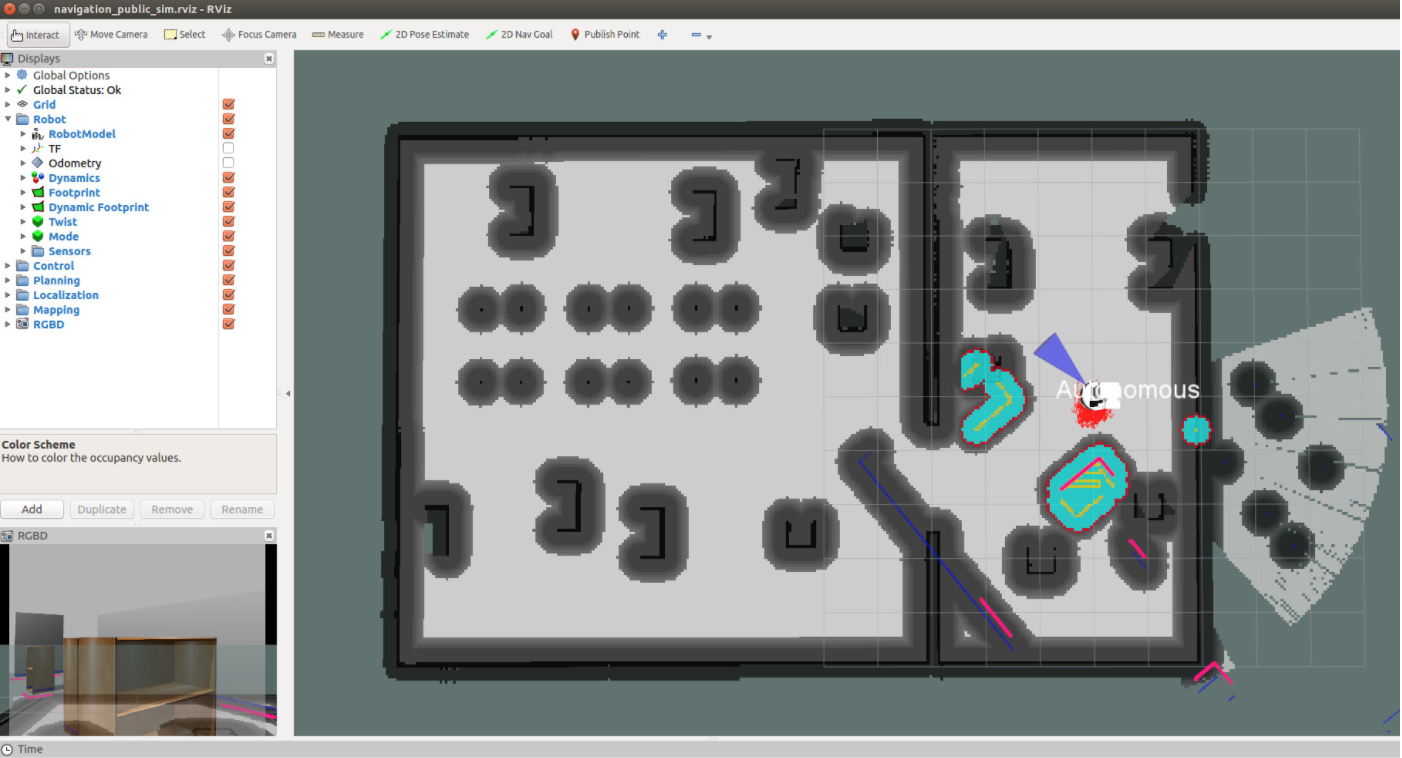
\includegraphics[width=\linewidth]{images/RVIZ_screenshot.png}
\end{center}
\caption{RVIZ in action.}
\label{fig:rviz_screenshot}
\end{figure}

\section{TIAGO}

TIAGO, a robot by PAL Robotics, is a the main and only robot used throughout the project given its characteristics and sensory devices treated in the coming sections. 

TIAGO is a service robot, designed to work in indoor environments \cite{website:TIAGo}, hence fitting our project aim of creating a ROS package for a robust human pose estimation which can be used to maneuver and interact around and with humans, although not limited to it only.

Moreover, TIAGO's size and technical features make it an ideal platform for the project, combining many of the necessary aspects for the positive outcome of the task, including RGB-D camera for 2D person detection and depth estimation, Laser range finder for person's leg detection and a Differential-drive base to move around the environment.

\begin{figure}[!htbp]
\begin{center}
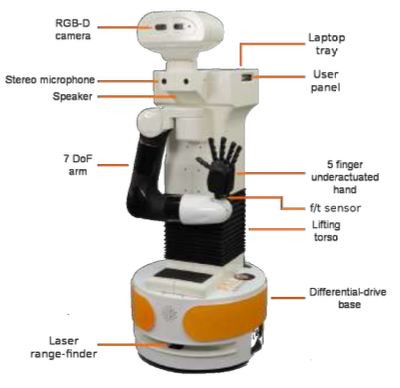
\includegraphics[width=3cm,height=4cm,keepaspectratio]{images/tiago_components.png}
\end{center}
\caption{TIAGO and its components (Image from PAL ROBOTICS \cite{website:TIAGOWEBSITE}).}
\end{figure}

\subsection{RGB-D}

The RGB-D sensor found on TIAGO, like other similar sensors such as the Kinect, provides both colour information as well as the estimated depth for each pixel in the two dimensional colour image.

To achieve this, TIAGO uses an RGB camera and a special camera sensor. In fact, the sensor firsts projects an infrared speckle patters which is ultimately captured by an infrared sensor component in it, and compared part-by-part to reference patterns stored in the device. The capture patterns are of known depth \cite{paper:RGB-D}.

A further step is still needed to obtain the corresponding depth in the RGB image, which is to correlate the data provided by the infrared sensor to a calibrated RGB camera, known as the Point Cloud, a three dimensional space collection of points \cite{paper:RGB-D}.

TIAGO already comes with an RGB-D camera integrated. An Astra model with a minimum and maximum sensor range of 0.6m and 8m.

\subsection{Lasers}

Laser-range finders is another important sensory device for this project. This technology is based on beam reflection and the time of flight.

The laser sends a pulse of light to target and measures the time it takes for the reflection to come back, i.e. the reflection \cite{website:lasers}. Therefore, by knowing the speed at which the beam travels (speed of light) and the time takes for the pulse of light to be emitted and come back, the distance is easily computable using the velocity equation.

TIAGO comes with an integrated laser-range finder with a range of 0.05-25 m and a 180 degree field of view. The frequency of the signal is of 15Hz.

\section{Human Detection}

Given the final objective of creating a ROS package able to estimate humans' position in the environment, a human detection module able to perform such detections on the available RGB sensory data is critical to the good development of the project.

Human detection is a popular and challenging task, given the wide range of features to be considered: skin colour and adopted human pose among others. Therefore, two possible ways of achieving the task have been identified. The first one uses a combination of image gradients and Support Vector Machine (SVM) machine learning model to classify whether humans are present in the image. The second approach is based on deep neural networks, and their ability to carry on object detection with high accuracy.

The two approaches will be considered in this chapter only from a theoretical and algorithmic point of view, thereby highlighting the mechanics of both models and the claimed accuracy and performance results from the respective papers. A more thorough experimentation will be carried on these during the implementation sprints, and a more in depth review will be given in terms of actual performance in the Implementation chapter.

\subsection{HOG (Histogram of Oriented Gradients)}

The Histogram of Oriented Gradients or HOG uses the below shown chain of feature extraction for the classification task.

\begin{figure}[!htbp]
\begin{center}
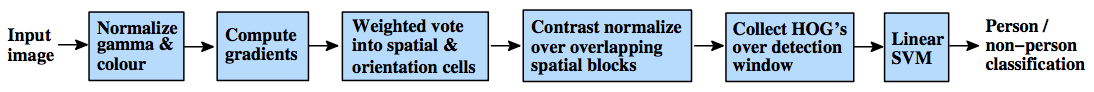
\includegraphics[width=\linewidth]{images/hog_chain.png}
\end{center}
\caption{HOG classification chain (Image taken from: \cite{paper:dalal2005histograms})}
\label{fig:hog_chain}
\end{figure}

The method carries its evaluation on contrast-normalised images to obtain well-contrasted images, as lighting variations and intensities are a key variable for a successful classification. After the input image has been normalised, local histograms of image gradient orientations are extracted by a sliding detection window over the image. The computed vectors are then added to the overall histogram used to identify the presence of humans in the image through a classification task run on SVMs, based on the idea that object appearance and shape can be characterised by the distribution of local intensity gradients and the edge directions \cite{paper:dalal2005histograms}.

The histogram based representation does offer some advantages, mainly it is robust to geometric and photometric transformations. Moreover possible translations or rotations do make little difference if these are smaller than the orientation bin size \cite{paper:dalal2005histograms}.

The descriptor has been tested on the MIT pedestrian database \cite{paper:dalal2005histograms} where it received  perfect detection results and on a custom dataset where instances are standing, but do appear on a variety of orientations and backgrounds however still outperforming other models like Haar Wavelets and PAC-SIFT \cite{paper:dalal2005histograms}.

In conclusion, from the results presented in the paper, the HOG based human detection task should well-perform in the task of detecting humans in RGB data in a reasonable computational time as the image to be searched will be of contained resolution.

\subsection{Deep Learning}

Deep learning is a subset of Machine Learning which has became a common approach to solve computer vision problems, since AlexNet in 2012 managed to improve object-detection accuracy using deep neural networks thanks to the increased availability of training data and most importantly the boost in performance of GPUs computations.

Yann Lacun, Yoshua Benjo and Geoffrey Hinton defined deep learning as a computational model composed of multiple processing layers able to learn the representation of data with multiple levels of abstraction \cite{paper:lecun2015deep}. Such methods have drastically improved the state-of-the-art in tasks like speech recognition, object recognition and object detection by iteratively discovering large data sets' structure using the backpropagation algorithm which helps the neural network update its parametric parameters \cite{paper:lecun2015deep}.

In particular three main models have been identified, able to perform object detection at a high level of accuracy:

\begin{enumerate}
  \item YOLO (You Only Look Once) \cite{paper:YOLO}
  \item Faster R-CNN \cite{paper:FRCNN}
  \item SSD (Single Shot Multibox Detector) \cite{paper:SSD}
\end{enumerate}

However, given the subtle difference in the classification accuracy of the aforementioned neural networks, the SSD model has been chosen out of the three for its computational efficiency and therefore its speed of detection as well as its ease to be embedded in a system. Moreover, the mobileNet version of the model will be used for its optimisation behaviour on power constrained devices.

\subsubsection{SSD Overview}

The SSD model is a single deep neural network able to detect various objects in a scene, by discretizing the output space with bounding boxes over different aspect ratios and scales per feature map (i.e. activation layer) \cite{paper:SSD}. During the feed-forward prediction process scores are generated for the presence of each object category in each bounding box along with an adjustment to the bounding boxes' to better match the object shape \cite{paper:SSD}. The network also combines various feature maps predictions with different resolutions to handle objects of various sizes. Moreover, the network classification process is simpler than other state-of-the-art models such as Faster R-CNN, as the former does not require proposal regions and subsequent pixel resampling stages, thereby encapsulating all required computations in a single network making of the SSD easy to train and straightforward to integrate into systems that require a detection component \cite{paper:SSD}, which is exactly our case.

\subsubsection{SSD Architecture}

Current state-of-the-art object detection systems are variances of the same detection process, which includes the following steps \cite{paper:SSD}:

\begin{enumerate}
  \item Hypothesize bounding boxes
  \item Pixel or features re-sampling
  \item Classification
\end{enumerate}

Although the above pipeline has proved to obtain great accuracy results, it has the major drawback of being too computationally expensive for real-time applications \cite{paper:SSD}. The SSD model improves upon Faster R-CNN \cite{paper:FRCNN} and YOLO \cite{paper:YOLO} by removing the need for bounding box proposals and the resampling process while still retaining the same accuracy performance using separate small convolutional filters applied at different aspect ratio detections \cite{paper:SSD}. These  filters are also applied to multiple feature maps from the later stages of the network in order to perform detection at multiple scales \cite{paper:SSD}.

\begin{figure}[!htbp]
\begin{center}
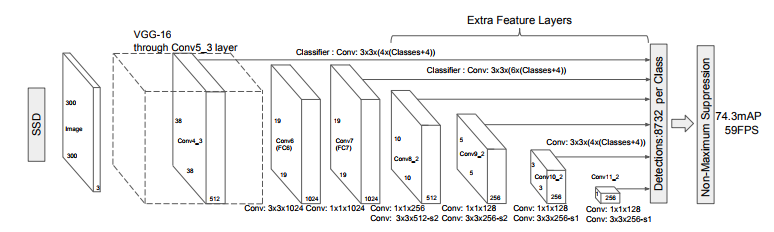
\includegraphics[width=\linewidth]{images/ssd_architecture.png}
\end{center}
\caption{SSD Model (Image taken from: \cite{paper:SSD})}
\label{fig:sshModel}
\end{figure}

The SSD architecture presents a standard base network (VGG-16) used for high quality image classification, upon which auxiliary layers are added to produce detections with the following key features:

\begin{enumerate}
  \item Multi-scale feature maps
  \item Convolutional predictors
  \item Default boxes and aspect ratios
\end{enumerate}

\textbf{Multi-scale feature maps}

Convolutional feature layers are added at the end of the truncated BASE network with the aim of progressively decreasing the input image size, hence allowing for detections at multiple scales \cite{paper:SSD}. Different convolutional models are used for each feature layer \cite{paper:SSD}.

\textbf{Convolutional predictors}

Each added feature layer on top of the base network can produce a fixed set of detection predictions using the previously mentioned convolutional filters \cite{paper:SSD}. Generally speaking a feature layer of size m x n with p channels requires a 3 x 3 x p kernel to produce either a score for a category or a bounding box offset relative to a default box position for each feature map location \cite{paper:SSD}.

\textbf{Default boxes and aspect ratios}

A set of default bounding boxes is associated for each feature map cell, for multiple feature maps at the top of the network (straight after the base network truncation \cite{paper:SSD}. At each feature map cell the offsets relative to the default box shapes as well as the per-class scores indicating the presence of a class instance in each of those boxes \cite{paper:SSD}. Specifically, for each box out of k, the \textit{c} class score is computed as well as the 4 offsets (for each discretized point of the original image 4 bounding boxes are draw with different aspect ratios) \cite{paper:SSD}.

\begin{figure}[!htbp]
\begin{center}
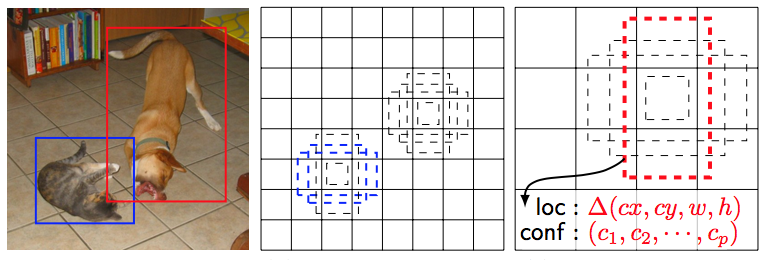
\includegraphics[width=\linewidth]{images/gt_boxes.png}
\end{center}
\caption{Ground truth, feature maps, offset computation(Image taken from: \cite{paper:SSD}).}
\label{fig:ssdGT}
\end{figure}

\subsubsection{MobileNets}

MobileNet provides an efficient network architecture in order to build small and low latency models that can be easily embedded in vision applications running on limited devices \cite{paper:MobileNets}. In fact, although the SSD model is relatively computationally lightweight compared to other state-of-the-art models it is still not enough to carry real-time detections on computationally limited platforms.

The MobileNet structure is built on top of a depthwise separable convolutions except for the first layer which is full convolutional layer \cite{paper:MobileNets}. Such a simplistic approach permits the further discovery of possible network topologies for a better performance overall. The MobileNet architecture is preseted below:

\begin{figure}[!htbp]
\begin{center}
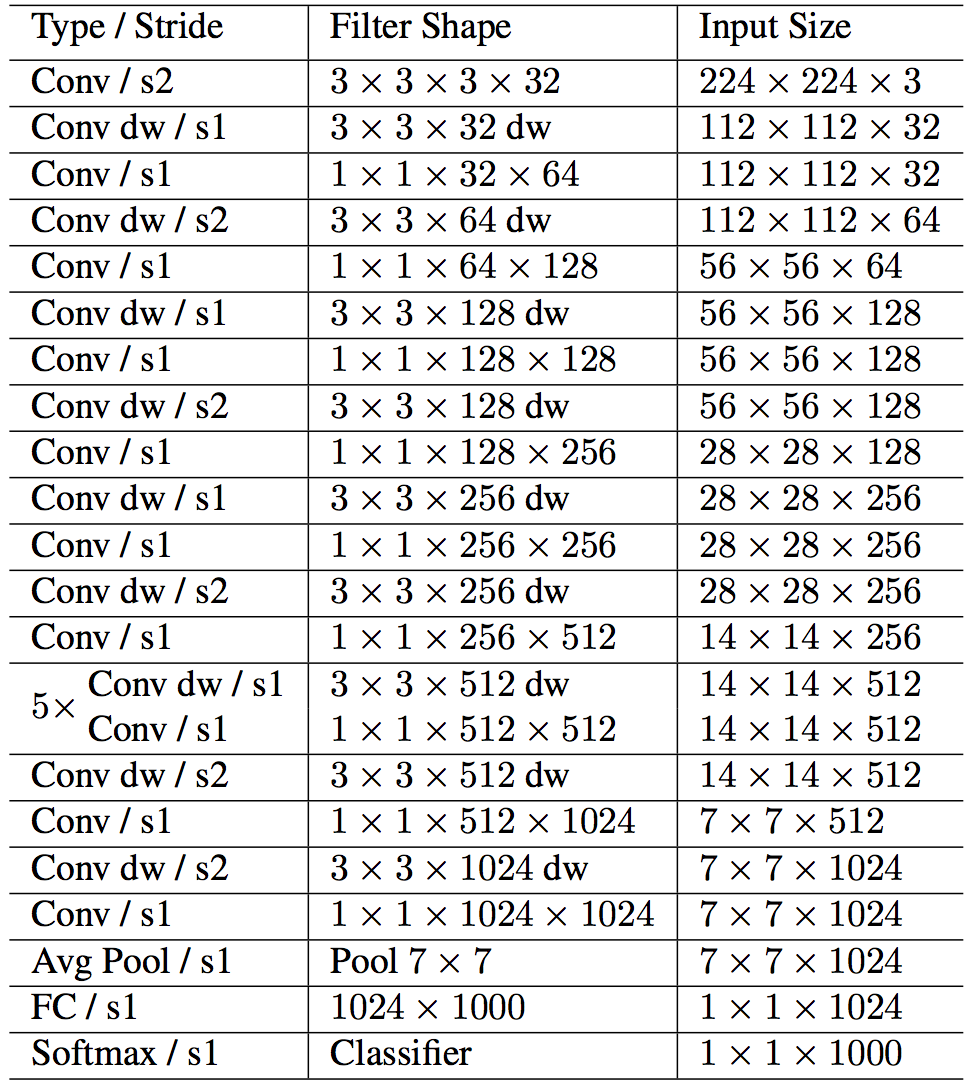
\includegraphics[width=7cm,height=9cm,keepaspectratio]{images/mobileNet_structure.png}
\end{center}
\caption{MobileNet Architecture (Image taken from: \cite{paper:MobileNets}).}
\end{figure}

Each component in the network is followed by a batch-normalization and a rectified linear unit with the sole exception of the final layer which feeds directly into the softmax layer for the classification \cite{paper:MobileNets}. Furthermore, the down sampling is handled with strided convolutions in the depthwise convolutions as well as in the first layer \cite{paper:MobileNets}, while a final average pooling does reduce the overall spatial resolution to 1 before the fully connected layer \cite{paper:MobileNets}. In total the MobileNet counts 28 layers.

\begin{figure}[!htbp]
\begin{center}
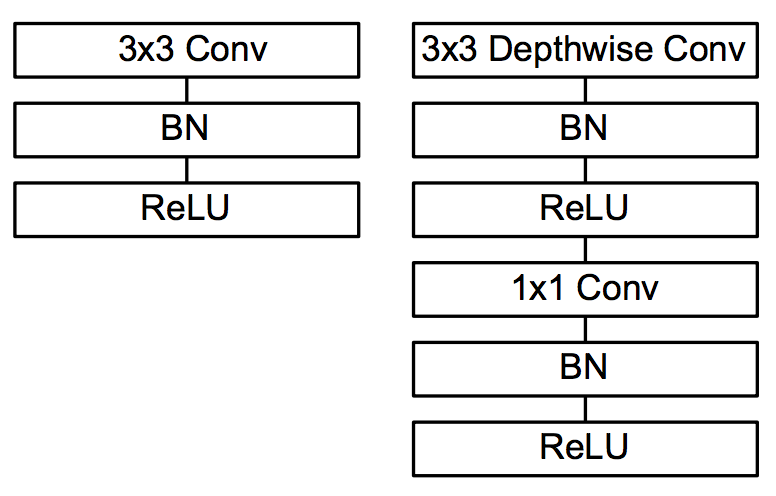
\includegraphics[width=7cm,height=9cm,keepaspectratio]{images/mobileNet_contrast.png}
\end{center}
\caption{Standard convolutional (left), Depthwise Separable convolutions (right) (Image taken from: \cite{paper:MobileNets}).}
\end{figure}

\subsubsection{Depthwise Separable Convolution}

The depthwise separable convolutions is a factorized convolution which factorizes a standard convolution into a depthwise convolution and a 1x1 convolution called pointwise convolution \cite{paper:MobileNets}.

The main difference between a usual convolution and the depthwise one is that the former applies both a filtering and combination procedure to the set of inputs into a new set of outputs in a single step \cite{paper:MobileNets} while the latter splits the procedure into two separate layers. This separation drastically reduces the computation and model size. The figure below shows a standard convolution (a), a depthwise convolution (b) and a 1x1 pointwise convolution (c).

\begin{figure}[!htbp]
\begin{center}
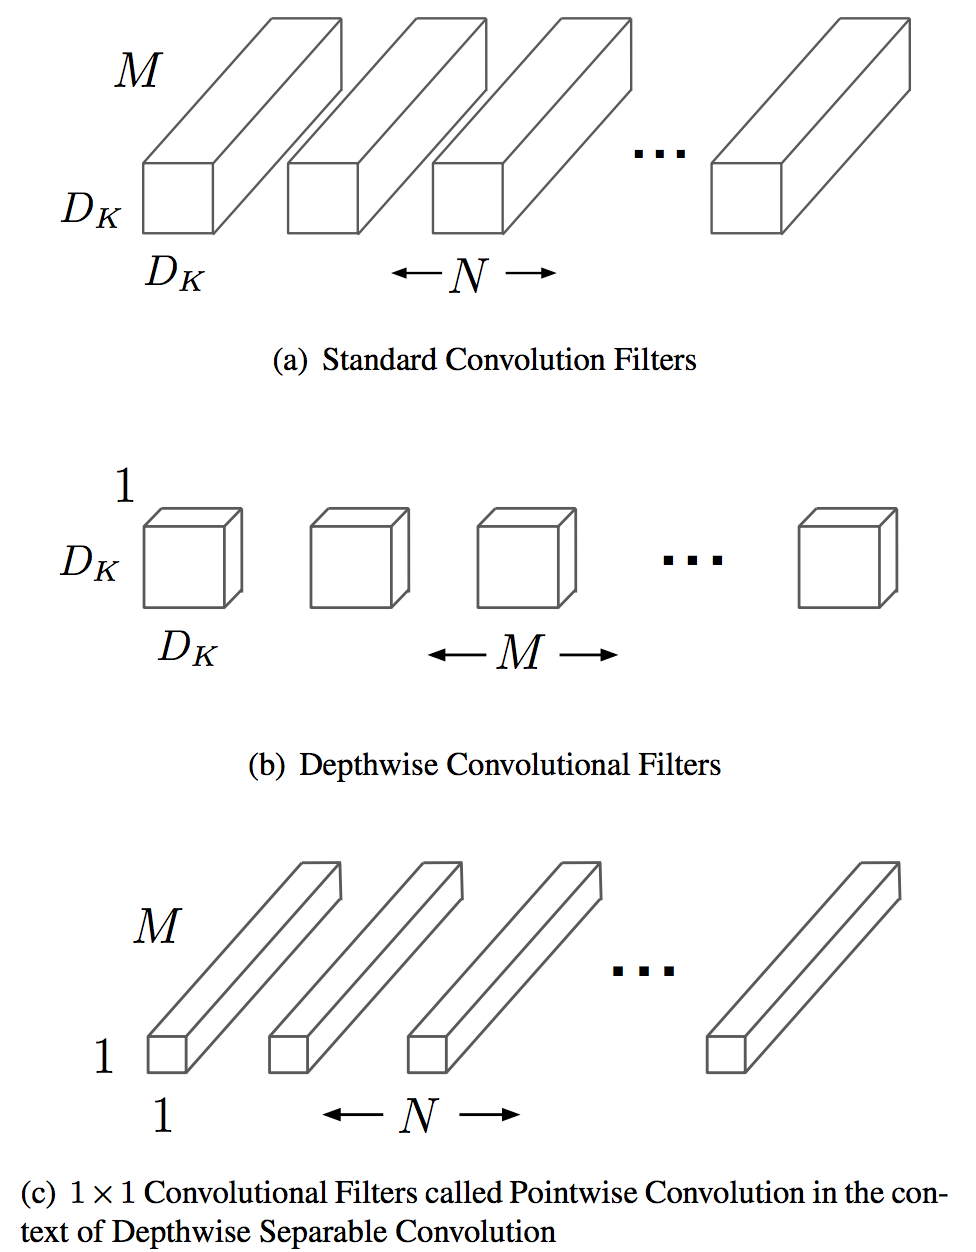
\includegraphics[width=5cm,height=7cm,keepaspectratio]{images/convolutions.png}
\end{center}
\caption{Convolution transformation (Image taken from: \cite{paper:MobileNets}).}
\end{figure}

\subsubsection{Width and Resolution Multipliers}

The basic mobileNet architecture already offers a better efficiency by being smaller and with a lower latency than the usual networks. Nonetheless, many times specif applications require a model which is even smaller and less computationally expensive. The width and resolution hyper-parameters serve exactly this.

The width multiplier defined with the greek letter \textit{alpha} has the role to thin the network layers uniformly \cite{paper:MobileNets}. Usual values for \textit{alpha} are between 0 and 1, with 1 being the model baseline for mobileNet. Moreover, the smaller the parameter gets, the smaller the model will be and hence the less accurate, therefore a trade off has to be found.

The second hyper-parameter to reduce the computational cost of a general neural network is the resolution multiplier defined with the greek letter p \cite{paper:MobileNets}. The parameter is directly applied to the input image and the internal representation of every layer is subsequently reduced by the same multiplier \cite{paper:MobileNets}. Typical values for p are between 0 and 1, with 1 being the mobileNet baseline.

Both parameters reduce the computational cost quadratically.

\begin{figure}[!htbp]
\begin{center}
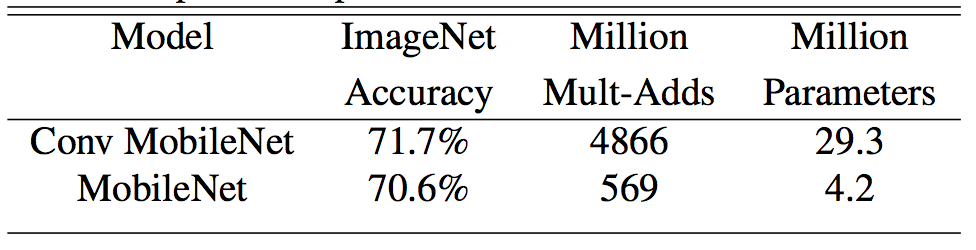
\includegraphics[width=10cm,height=10cm,keepaspectratio]{images/mobileNet_table.png}
\end{center}
\caption{Full vs Depthwise convolutions performance (Image taken from: \cite{paper:MobileNets}).}
\end{figure}

\section{Distance Estimation}

To be able to estimate the position of a person in the final ROS package the only RGB detection is not enough. The distance from the robot to the person is required.

Two main possible approaches have been identified to solve the problem. The first one consists using the RGB-D sensor which comes integrated on TIAGo and which has been presented in Chapter1. The second viable approach consists in Triangulation, a common vision technique to obtain depth from two or more viewpoints.

\subsection{RGB-D}



\subsection{Triangulation}

\section{Leg Detection}
  \chapter{Person Detection Development}
\label{chapter3}

\section{Deep Learning Approach}

To develop the person detection module two different approaches were presented in Chapter2. The HOG algorithm and deep-learning based models. Both methods make use of the incoming RGB data from the on-board RGB-D sensor.

The Histogram of Oriented Gradients (HOG) and its possible variances, such as the Oriented Histograms of Flow and Appearance (OHFA) and the AdaBoosted version, was the first natural choice for the task, due to its simplicity in the integration as the method was already implemented in the OpenCV library. However, the method's performance was acceptable only in close to perfect conditions due to the mechanics of the algorithm. Mainly when people are clearly visible in a seated or standing position, within sparse environments, and with no or little occlusions. False positives were also another problem encountered as shown in the pictures below. Moreover, the sliding window technique used by the method is rather inefficient as it has to search through the whole frame, making it computationally expensive for large ones.

On the other hand the deep-learning model proved to work really well under circumstances where HOG failed. Such as when people are standing or seated with partial body occlusion which is common in indoor environments. Moreover, each detection comes with the relative probability of the latter being a person. Allowing to discard detections with low confidence, something that was not possible with the HOG algorithm. Hence the decision to choose a deep leaning approach for the task.

\begin{figure}[H]
    \begin{subfigure}{.5\textwidth}
        \centering
        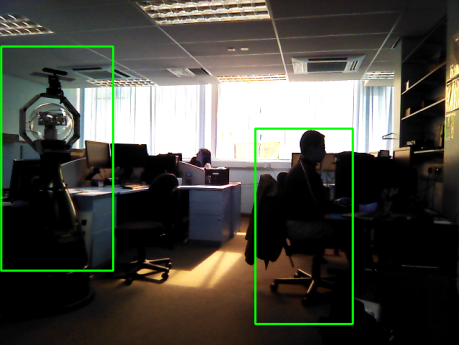
\includegraphics[width=.85\linewidth]{images/chapter3_hog.png}
        \caption{HOG detection with false positive.}
	\end{subfigure}
    \begin{subfigure}{.5\textwidth}
        \centering
        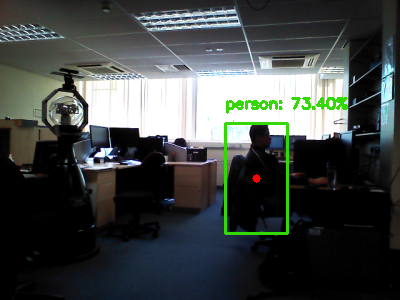
\includegraphics[width=.85\linewidth]{images/chapter3_dnn.png}
        \caption{SSD detection with no false positives.}
	\end{subfigure}
    \label{fig:hog}
\end{figure}

\subsection{Stack}

The stack used for the development of the detection module includes the Python programming language and the OpenCV library.

The choice to use Python derives from the nature of the project. Being it an \textbf{Exploratory Software} product there was a lot of prototyping phases to it before settling for particular approaches or methodologies. Making of Python a natural choice for its dynamic behaviour and its ease of implementation. Moreover, both the ROS interfaces as well as the OpenCV library used offered Python bindings to call their relative APIs.

Version 3 of the Python programming language was used in particular along with OpenCV 2.4.8 and 3.3.0 to relatively access Indigo's \textbf{CvBridge} interface modules and the \textbf{dnn}\footnote{deep-neural-network} module to work with the serialised SSD network.

Two different versions of OpenCV were used because the ROS indigo version comes with standard static bindings for version 2.4.8 of the computer vision library. No easy install was also available to upgrade to the latest version of OpenCV, required for the dnn module, which would still be compatible with Indigo's CvBridge interface. A ROS distro upgrade wasn't an option either, given the need of the Indigo version for compatibility with TIAGO. The only remaining choice was to directly deal with a source installation and possibly fix the broken stating linkages along the way, which due to time constraints was avoided. Virtual environments were instead used to solve the issue.

\subsubsection{Virtual Environment Set-up}

A virtual environment is a cooperatively isolated runtime environment that allows Python users and applications to install and upgrade Python distribution packages without interfering with the behaviour of other Python applications running on the same system \cite{website:virtualEnv}.

To make use of such an environment some steps need to be taken. First of all the python package installer (pip) has to be installed if not already available and upgraded to the latest version. The last point is of particular importance as to access later on the latest version of OpenCV through pip, this has to be upgraded to the latest version as well.

The next step consists in installing the virtual-environment and the virtual-wrapper via pip which offers a higher level interface for the former to ease the creation of a personalised environment. However, before proceeding to the actual creation of the environment, the package installer cache needs to be cleaned as shown below, in order to avoid conflicting issues with older versions present within it.

\begin{lstlisting}[language=bash]
$ sudo rm -rf ~/.cache/pip
\end{lstlisting}

Next is the actual creation of the virtual-environment using the \textbf{mkvirtualenv} command made available through the virtual-wrapper package, that takes as a compulsory argument the name of the environment, in this case harn, and as an optional one the Python version to be installed within it. In this occasion Python3 was installed as it is a compulsory requirement for the OpenCV version to be installed. The creation command is as follows:

\begin{lstlisting}[language=bash]
$ mkvirtualenv harn -p Python3
\end{lstlisting}

Finally, the virtual-environment needs to be made accessible through simple bash commands, so as to activate and de-activate the environment easily. For this, the created virtual environment is exported in the \textbf{.bashrc} file which makes it available to all future bash sessions upon start. The export command is as follows:

\begin{lstlisting}[language=bash]
$ export WORKON_HOME=$HOME/.virtualenvs
\end{lstlisting}

\subsubsection{OpenCV 3.3.0 Installation}

Once the environment is set-up, activating and de-activating it is as easy as a matter of calling the \textbf{workon} and \textbf{deactivate} commands, also made available by the virtual-wrapper package. Upon activating the custom environment, the required OpenCV version can be installed using a simple pip install as shown below. The installation makes available the required dnn module.

\begin{lstlisting}[language=bash]
$ workon harn # This activates the environment called harn
(harn)$ pip install opencv-contrib-python # Installs OpenCV 3.3.0
(harn)$ deactivate # This de-activates the environment
$ # Now the environment is not active anymore
\end{lstlisting}

Whenever the detection module needs to be executed this takes place in the isolated and activated harn virtual-environment. Where the latest OpenCV and Python3 versions are made available. The remaining modules are run in normal environments.

\subsection{Module design}

The final solution design was affected by the Indigo-OpenCV compatibility issue presented before. More precisely, the detection module is not able to convert beforehand the RGB data incoming from the subscription into an OpenCV specific format, such as MAT, as the CvBridge interface is incompatible with the latest version of the computer vision library.

Hence, the decision to split the single detection module into two different ones. With one component performing the conversion and the other the detection. The conversion module is accountable for the conversion of the raw coloured image into a MAT format, using the standard OpenCV 2.4.8 version and the compatible CvBridge interface. The detection module, instead, is solely responsible to perform the detection process on the converted image.

\subsection{OpenCV conversion}

The conversion component is implemented as a collection of routines in the \textbf{cv\_conversion.py} file made available in project's GitHub repository. The steps to the conversion task are the following:

\begin{enumerate}
  \item Image topic subscription
  \item Callback conversion
  \item Conversion storage
\end{enumerate}

\subsubsection{Image Topic Subscription}

This step consists in subscribing to the raw stream of data published by the robot's RGB-D sensor. However, before being able to create the subscription a node has to be created. In fact, by making use of the ROS middleware, all communications happen over topics which allow the instances of the ROS graph, called nodes, to interact with each other by publishing or subscribing over the topic channels. 

To create the node the \textbf{rospy} library and the \textbf{init\_node}, whose arguments taken are two, are used. The parameters are the node's name so that it can be distinguished amongst the possible hundreds of nodes running in the graph, and a boolean flag, which if true, adds random numbers at the end of the node's name to ensure its uniqueness \cite{website:nodes}. The following is the node creation call:

\begin{lstlisting}
rospy.init_node('cv_conversion', anonymous=True)
\end{lstlisting}

Once the node is created, the subscription is a matter of using the \textbf{Subscriber} routine available through the \textbf{rospy} library. The Subscriber method takes three arguments. The first one is the topic string where the raw RGB data are being published by the robotics system in use, in this case \textbf{xtion/rgb/image\_raw}. The second argument is the message type being received through the subscription. ROS offers many built-in messages type, but for this particular subscription the data received is a standard\_msg/Image, which before being used has to be imported at the top of the script. The third and last argument is the callback function called once the data is received and whose task is to manipulate the raw information. The subscription call is as follows:

\begin{lstlisting}
rospy.Subscriber("/xtion/rgb/image_raw", Image, toMat)
\end{lstlisting}

\subsubsection{Callback Conversion}

The callback function has the task to manipulate the received data through the subscription. A callback function called \textbf{toMat} is defined which takes as argument the image\_raw data afterwards converted. Before describing the conversion step, it is interesting to note how the data is actually passed to the function. In fact, everything is handled by the Subscriber method which receives the data and does the call to the function reference passing the information received as an argument. Therefore no step in between is actually required.

The data conversion uses the \textbf{imgmsg\_to\_cv2} routine which is a method belonging to the CvBridge module. The function takes two arguments, the ROS image message to be converted and the encoding to convert it into. In this case, these are the image\_raw passed to the callback function and bgr8. The conversion call is as follows:

\begin{lstlisting}
cv_image = CvBridge().imgmsg_to_cv2(image_raw, 'bgr8')
\end{lstlisting}

\subsubsection{Conversion storage}

Lastly the converted image has to be made available to the detection module for the detection process. This is exactly why the conversion was stored in a variable instance named \textbf{cv\_image}, as this is passed as a parameter to a second function whose task is just to save the image to the disk. A function called \textbf{store} is defined, that takes as input the OpenCV image and calls the \textbf{imwrite} routine, available through OpenCV, to store the converted image in the specified path. The function call is as follows:

\begin{lstlisting}
cv2.imwrite(PATH + "/data/converted/image.png", cv_image)
\end{lstlisting}

where \textbf{PATH} is a constant variable storing a dynamic path to the folder used for the storage, so that no issues arise if the package is cloned in different paths by different users. The \textbf{path} python library is used to facilitate the path planning. The variable definition is as follows:

\begin{lstlisting}
PATH = str(Path(os.path.dirname(os.path.abspath(__file__))).parents[0])
\end{lstlisting}

\subsection{OpenCV detection}

The detection module, differently from the conversion component, is implemented as a class in the \textbf{human\_detection.py} file made available in the GitHub repository for the project. The steps to the detection process are the following:

\begin{enumerate}
  \item Model de-serialisation
  \item Image loading
  \item Feed-forward
  \item Process detections
  \item Message publication
\end{enumerate}

\subsubsection{Model De-Serialisation}

The original MobileNet version of the SSD model presented in Chapter1 was trained using Google's TensorFlow machine learning library by Howard et al. \cite{paper:MobileNets}. However, the version used for the project embedding makes use of the Caffe version trained by chuanqi305 \cite{website:chuanqi305}.

The trained model is able to detect over 20 different objects in images and is made available through serialised files that include the the \textbf{MobileNetSSD\_deploy.caffemodel} as well as the \textbf{MobileNetSSD\_deploy.prototxt}. The former defines the internal states and parameters for each layer, while the latter describes the architecture of the network, such as the input dimensions, the number of layers and the base network used as well as the activation function for every feature map.

Given that the neural network is serialised a de-serialisation process is required. The dnn module introduced in version 3.3.0 of OpenCV is used to load the serialised Caffe model. Caffe trained networks are not the only accepted ones, as the dnn library can work with a variety of other machine learning frameworks, including TensorFlow and Keras.

The de-serialisation or loading process does happen at the constructor level of the class that implements the detection module. In fact, by using an object-oriented design a single instance can be used to handle all detection requests afterwards. Therefore avoiding to load the model multiple times as only one de-serialisation is needed at the instantiation level. To perform the loading the \textbf{readFromCaffe} routine belonging to the dnn module's namespace is called, to which both the prototxt and .caffemodel files are passed as arguments as follows:

\begin{lstlisting}
self.net = cv2.dnn.readNetFromCaffe("prototxt.txt", "model.caffemodel")
\end{lstlisting}

\subsubsection{Image loading}

A further step is required before running the feed-forward routine made available through the de-serialisation of the model. This consists in actually loading the image to be fed to the neural network which was previously converted by the conversion module. OpenCV's \textbf{imread} routine is used for the task, whose only parameter is the path to the image. The function call is as follows:

\begin{lstlisting}
cv_image = cv2.imread(self.path + "/data/converted/image.png")
\end{lstlisting}

\subsubsection{Feed-forward}

The feed-forward process consists in feeding the loaded image to the neural network, which runs the detection algorithm to find people within the input image. However, before running the algorithm a couple more variables need to be initialised. These are the target variable, that identifies the class category of interest to be detected. In this case corresponding to the value 15 as people is the 15th category out of the 20 available. And the confidence variable which determines the minimum probability that a detection needs to have so as not to be filtered out. The confidence value of 0.5 turned out to be a good one. The array of targets containing all the possible categories is also defined.

Input-wise, the network accepts multiple image colour spaces, including grayscale and RGB with the only constraint that the input dimensions are of 300x300 pixels. This means that the original input has to undertake a pre-processing step to scale it down to the required size, as the original is of 640x480. Moreover, mean-subtraction and scaling are also applied to the resized image via the \textbf{blobFromImage} function to further improve the chances of obtaining a correct detection \cite{website:blobFromImage}. The input preparation logic is as follows:

\begin{lstlisting}
# Resize image
resized = cv2.resize(frame, (300, 300))
# Apply pre-processing steps
blob = cv2.dnn.blobFromImage(resized, 0.007843, (300, 300), 127.5)
\end{lstlisting}

The rest of the detection process is straightforward, as it is a matter of passing the pre-processed image to the network and run the feed-forward process. The dnn module offers routines for both of these tasks, by respectively calling the \textbf{setInput} method on the network instance and passing it the blob object as shown below:

\begin{lstlisting}
self.net.setInput(blob)
\end{lstlisting}

The detections result can then be obtained by running the \textbf{forwards} method on the same network instance as follows:

\begin{lstlisting}
detections = self.net.forwards()
\end{lstlisting}

\subsubsection{Process Detections}

The network is trained to recognise twenty different categories. This project, however, is only interested in detecting people presence in the image without much concern about any other object. Hence, within the iteration that loops over the detections returned by the feed-forward process, which is a multi-dimensional array, a conditional statement is added that checks whether the detection ID is equal to the previously defined target variable. The confidence variable, also previously defined, is also used within the same conditional statement to check that the person labelled detection is over a certain threshold by using an AND connective.

\begin{lstlisting}
# Loop over the detections
for i in np.arange(0, detections.shape[2]):
	# Get detection probability
	confidence = detections[0, 0, i, 2]

	# Get ID of the detection object
	idx = int(detections[0, 0, i, 1])

	# Filter out non-human detection with low confidence
	if confidence > self.confidence and idx == self.target:
    	# Rest of the logic goes in here
\end{lstlisting}

\textbf{Message publication}

Many are the information made available by the detections result tensor. The confidence and the categorical class for each detection are just two of these. The other important detail used in the project is the actual position of the person in the RGB frame, which for each detection is in terms of its top-left and bottom-right point. Hence, the width, height and consequently the centre point of the bounding-box around the detected person can be easily computed and published over a topic.

The publisher-subscriber is the main ROS communication paradigm, where a node can publish over a particular topic different messages and subscribe to as many others. Therefore, to allow interested users to have access to such information, the centre point of the detections obtained from the feed-forward process are made available over a topic called \textbf{detections}. This publishes a custom message defined for the project named \textbf{Detections}. The \textbf{Publisher} routine is used for this, which takes as the first argument the topic's name, followed by the message type and lastly the buffer size as follows:

\begin{lstlisting}
self.detection_pub = rospy.Publisher('detections', Detections, queue_size=5)
\end{lstlisting}

ROS already comes with standard data-types such as int, float and many others. Nonetheless, the creation of a new custom message to compactly store related data is straightforward. First a \textbf{msg} folder is created at the root level of the package, which will store the defined messages. Two messages are then created within the msg folder, one called \textbf{Detection.msg} which holds the details of the single detection, and another named \textbf{Detections.msg} that acts as a collection of all the details for all the detections that passed the if statement criteria. The two message definitions for the Detection.msg(left) and the Detections.msg(right) are shown below:

\begin{multicols}{2}
  \begin{itemize}
    \item int32 ID
    \item int32 centre\_x
    \item int32 centre\_y
  \end{itemize}

  \columnbreak

  \begin{itemize}
    \item Header header
    \item int32 number\_of\_detections
    \item Detection[] array
  \end{itemize}
\end{multicols}

The fields of the Detection message consist in three 32 bits integer fields. The ID one that will serve in later modules to correspond which distance or 3D position is to which detection, as well the centre\_x that stores the x-coordinate of the centre point of the detection and centre\_y for the y-coordinate. Publishing each detection message by itself would not make sense. Hence the need for the Detections message that has as fields a header storing information about the timestamp of the message, a 32 bits integer storing the number of the total detections for the input image and a collection of Detection messages. The custom messages before being available for usage need to be added to the CMAKE file at the root of the package and built using \textbf{catkin build}.

For each positive detection in the loop, a new Detection message instance is created and its fields are populated using Python's field access syntax. The ID takes the value of the current number\_of\_detections, which at first is 0 and is increased at every loop iteration, ultimately being set back to 0 at the end of the loop. The centre point of the detection's bounding-box is computed using the top-left and bottom-right information from the detections tensor for the specific instance, and its x and y coordinates are then stored in the relative fields. Every Detection object is then pushed to the Detections' array field using a simple append. The Detections message instance is a global one defined in the constructor, which gets re-instantiated at the end of each loop to clear it from the previous pushed content. The population is as follows:

\begin{lstlisting}
# Create Detection message
detection = Detection()

# Populate Detection message
detection.ID = self.number_of_detections
detection.centre_x = centre_ratio_point[0]
detection.centre_y = centre_ratio_point[1]

# Push Detection message to Detections array field
self.detections.array.append(detection)
\end{lstlisting}

At the end of each feed-forward request, the Detections message is published through the detections topic using the \textbf{publish} method on the publisher instance, which takes as its only argument the message to be published, in this case self.detections as follows:

\begin{lstlisting}
self.detection_pub.publish(self.detections)
\end{lstlisting}

An example output of the detections topic using the \textbf{topic echo} command is shown below:

\begin{figure}[H]
  \begin{center}
    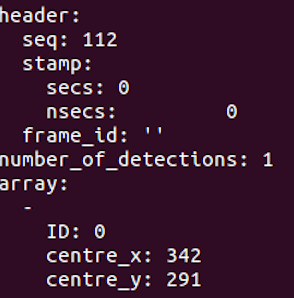
\includegraphics[width=0.5\linewidth]{images/chapter3.png}
  \end{center}
  \caption{Detections topic output.}
  \label{fig:det_topic}
\end{figure}


  \chapter{Final Solution Architecture \& Integration}
\label{chapter4}

\section{TODO}
  \chapter{Architecture \& Modules Integration}
\label{chapter5}

\section{Architecture}

\begin{figure}[H]
  \begin{center}
    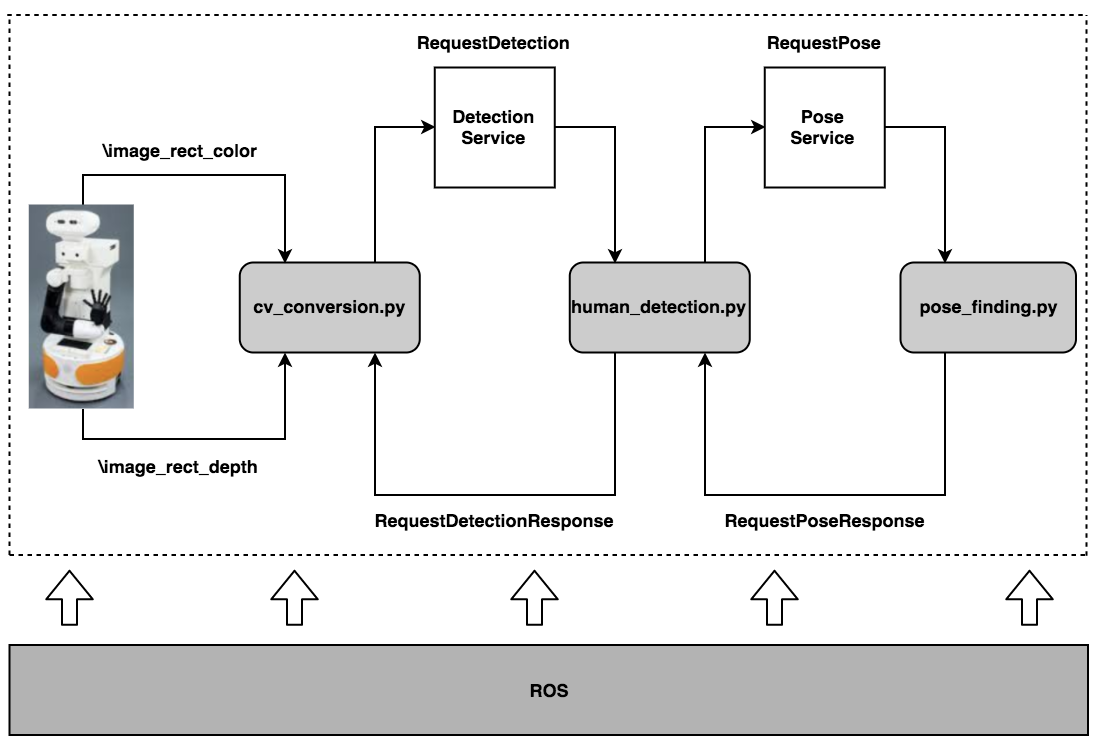
\includegraphics[width=\linewidth]{images/chapter6_architecture.png}
  \end{center}
  \caption{Project's architecture.}
  \label{fig:architecture}
\end{figure}

The final solution has three main components to it:

\begin{enumerate}
	\item The conversion script that converts the \textbf{image\_rect\_color} into an OpenCV format.
    \item The detection script that detects people in the converted frame.
    \item The pose script that computes the detection's distance and finds its 3D pose in the map frame.
\end{enumerate}

All of the components do sit on top of the ROS middle-ware whose utilities include ROS services, standard messages and publish-subscribe communication paradigms among others. Moreover, it is essential to have a ROS master available for the package to work as this handles the topics and makes available the required topics such as the rectified coloured image and the rectified depth-image, where in this occasion these were made available by TIAGo's bring-up and its ROS master export in the development machine. 

Lastly ROS services were used for module-intra-communication. Figure 5.1 gives an overview of how the communication happens and in which order between the various components.

\subsection{Communication Logic}

\subsection{Conversion}

The conversion module was implemented via a set of routines which are called by the main within the same file, which subscribes to the rectified colour and depth image, converts the former and sends a service request to the detection module, which will respond with a success or failure message (once the whole communication chain is resolved).

\subsection{Detection}

The detection module waits until the service request from the conversion script is received, and upon which it runs the feed-forward process, creates a detections message and passes this to the next module via a different service request.

\subsection{3D Pose}

Finally the pose module receives the request from the detection module, computes the distance for every detection its 3D pose in the map. Once done, a set of markers are published to RVIZ along with a custom poses message with the 3D pose for each detection, and a response notifying the success of failure of the process is sent back to the service caller.

\section{Modules Integration}

The original plan for the development consisted in having separate modules for each task that operate independently of each other, and that would have access to each others computations via the published topics. 

However, this had to be reconsidered when the pose and detection modules had to be integrated. In fact, given that the subscribed depth-image published by TIAGO's interface has a lower publishing rate then the coloured image, a synchronisation problem happened, where the wrong depth ROI\footnote{Region of Interest} was accessed because of the delay, which ultimately consisted in computing the wrong distance and therefore the wrong 3D pose.

\subsection{Time Synchroniser}

To solve the synchronisation issue an approximate time synchroniser was used. More precisely the \textbf{ApproximateTimeSynchroniser} routine made available by the message\_filters library allows the subscription to multiple topics whose callback function is called only when the timestamps differences are within a certain threshold. 

Therefore, two separate subscriptions called \textbf{rgb\_sub} and \textbf{depth\_sub} were made respectively to the raw rectified image and the rectified depth-image topics, in the \textbf{cv\_conversion.py} script, which consequently got chained together using the time synchronizer with a threshold error of at most 0.5 seconds, as shown below. Of course, the bigger the threshold, the greater the delay, hence a good empirical value had to be found. The synchronisation is then binded to a callback function called \textbf{processSubscriptions} using the \textbf{registerCallback} routine, also made available by the message\_filters library as follows.

\begin{lstlisting}
import message_filters as mf
ats = mf.ApproximateTimeSynchronizer([rgb_sub, depth_sub], slop=0.5)
ats.registerCallback(processSubscriptions)
\end{lstlisting}

\subsection{ROS Services}

Two choices were available for the module-intra-communication, by either using standard publish-subscribe communication or an RPC based style via services. 

The original idea was to use the former type of communication, as it would allow a more flexible and modular usage of the package given that if a user only wants to use a specific component of the package, only the required module would have to be executed. However, due to the RGB-depth synchronisation problem, and the fact that the subscriptions are both made in one place (the conversion script) and not in their relative module as originally planned (so rgb\_sub in the conversion module and depth\_sub in the pose module) the latter type of communication via ROS services was preferred for an easier message exchange. In fact, via a service mean, the collected ROS messages at subscription time can be passed forward to server nodes with simple \textbf{srv} files rather then having to publish them all over again.

Hence a \textbf{srv} folder is created in the same path as the msg folder at the root of the catkin package, in which two services are defined, a detection one called \textbf{RequestDetection.srv} that requests the feed-forward process to the detection module, and that has as a client the conversion component and as the server the detection one. A pose service named \textbf{RequestPose} is also declared, which requests the actual distance and 3D pose computation, and whose client is the detection module and server the pose component. The two service declarations for the RequestDetection.srv(left) and the RequestPose.srv(right) are as follows:

\begin{multicols}{2}
  \begin{itemize}
    \item sensor\_msgs/Image depth
    \item - - -
    \item string res
  \end{itemize}

  \columnbreak

  \begin{itemize}
    \item Detections detections
    \item sensor\_msgs/Image depth
    \item - - -
    \item string res
  \end{itemize}
\end{multicols}

A typical service message is made of a request and response declaration separated by a dotted line. 

In the case of the detection service the input passed through the service request by the conversion script is only the synchronised image, as the RGB image is stored on the disk. The response expected by the service is a string determining either the success of failure of the service, which is then printed to the console for the user to keep track of the process.

Similarly the pose service request expects as input the detections computed by the neural network as a Detections message, as well as the depth-image originally retrieved during the conversion process at the beginning of the chain. The response expected is again a string suggesting the failure or success of the process.

The service request are blocking, which means that the module is idled as it waits for the server to come up or the response message to come back, which is something to improve upon in the future.



  \chapter{Testing \& Evaluation}
\label{chapter6}

The testing process was made of two steps. First, an efficiency evaluation of the package was made to determine the computational time needed for the whole logic to run. Finally, each individual component in the package was separately tested in indoor environments, where such an interface could be made use of.

\section{Timing breakdowns}

Efficiency was an important attribute to the project since the early planning stage, as the solution is targeted towards real-time applications usage. In this section the timing measurements for each module are presented along with a small discussion about the average execution time and whether the original target was reached.

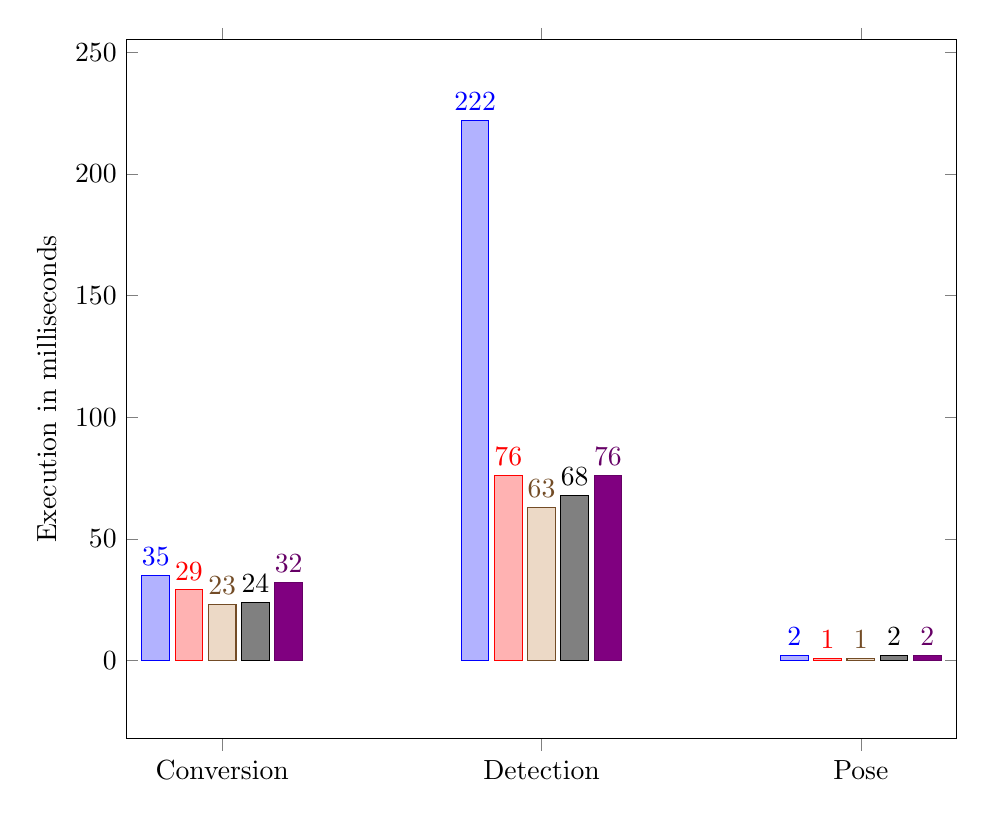
\begin{tikzpicture}
	\begin{axis}[
    	ybar,
        enlargelimits=0.15,
        legend style={at={(0.5,-0.15)},
        anchor=north,legend columns=-1},
        ylabel={Execution in milliseconds},
        symbolic x coords={Conversion, Detection, Pose},
        xtick=data,
        nodes near coords,
        nodes near coords align={vertical},
        width=\textwidth
        ]
        \addplot coordinates {(Conversion, 35) (Detection, 222) (Pose, 2)};
        \addplot coordinates {(Conversion, 29) (Detection, 76) (Pose, 1)};
        \addplot coordinates {(Conversion, 23) (Detection, 63) (Pose, 1)};
        \addplot coordinates {(Conversion, 24) (Detection, 68) (Pose, 2)};
        \addplot coordinates {(Conversion, 32) (Detection, 76) (Pose, 2)};
	\end{axis}
\end{tikzpicture}

From the histogram of the time breakdowns showed above, all of the modules do perform extremely efficiently. In particular, the conversion component takes on average \textbf{28.6 milliseconds} to finish the conversion step. Detecting people on the RGB frame, which is by far the most computationally expensive step, takes an average of only \textbf{101 milliseconds}. Finally, the 3D pose estimation module was unsurprisingly the fastest one, as it completes the computation in only \textbf{1.6 milliseconds}.

The average computational time for the package to carry out the estimation process is of only \textbf{43.7 milliseconds}. Therefore, the original objective of developing a ROS package usable in real-time can be considered met.

\section{Module Testing}

In this section the testing is primarily focused on the individual modules. In particular, the detection and pose module are tested in isolation to check their performance within indoor environments. Note that the conversion module is not tested as it does not have a real impact in the ultimate estimation.

\subsection{Person Detection}

The detection's module tests were carried in two different environments, one being the robotics lab at the University of Leeds whose lighting conditions are not the best and whose space is really crammed and cluttered with objects, and the long-room area which offers a sparse area with a good lighting conditions. Clutter, occlusions, scale and lighting conditions were the situations tested.

\subsubsection{Light conditions, Scale \& Clutter}

\begin{figure}[H]
    \begin{subfigure}{.5\textwidth}
        \centering
        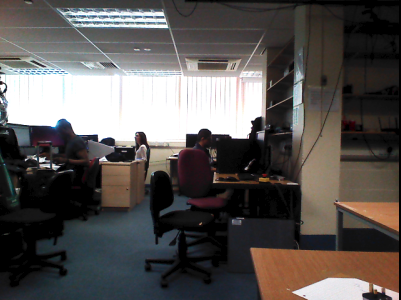
\includegraphics[width=.9\linewidth]{images/chapter6_clutter_light.png}
        \caption{Poor light condition and clutter.}
	\end{subfigure}
    \begin{subfigure}{.5\textwidth}
        \centering
        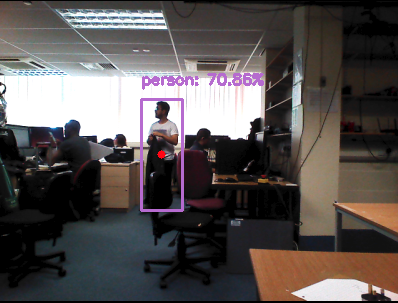
\includegraphics[width=.9\linewidth]{images/chapter6_clutter_light_detection.png}
        \caption{Detection in clutter.}
	\end{subfigure}
    \begin{subfigure}{.5\textwidth}
        \centering
        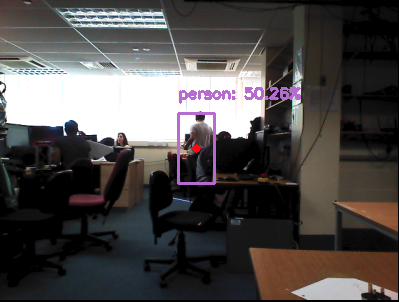
\includegraphics[width=.9\linewidth]{images/chapter6_clutter_light_detection_back.png}
        \caption{Detection in clutter (person showing back).}
	\end{subfigure}
    \begin{subfigure}{.5\textwidth}
        \centering
        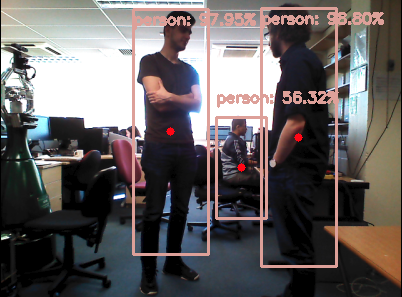
\includegraphics[width=.9\linewidth]{images/chapter6_clutter_standing.png}
        \caption{Multiple detections in clutter.}
	\end{subfigure}
\end{figure}

The outcomes of the detection module in poor lighting conditions are variable. In fact, Figure (a) shows a poor performance in the detection process as none of the three subjects in the picture were detected. However, this is not entirely to be attributed to the lighting conditions as the individuals are all partially occluded in the clutter of the lab.

Figure (b) and (c) show an improvement in the detection outcome when one of the individuals is standing in the room. Both situations present a difficult situation, as in (b) the subject has his lower-body covered by a jacket and in (c) the same person is standing showing only his back and still partially covered which determines the low confidence in the detection, which is only 50\%.

Figure (d) shows a robust detection result when the subjects are standing clearly even in poor lighting conditions and when not facing directly the camera. Moreover, the same figure shows how well the module handles detections at different scales by detecting a third seated person further down the room.

\subsubsection{Occlusions}

\begin{figure}[H]
    \begin{subfigure}{.5\textwidth}
        \centering
        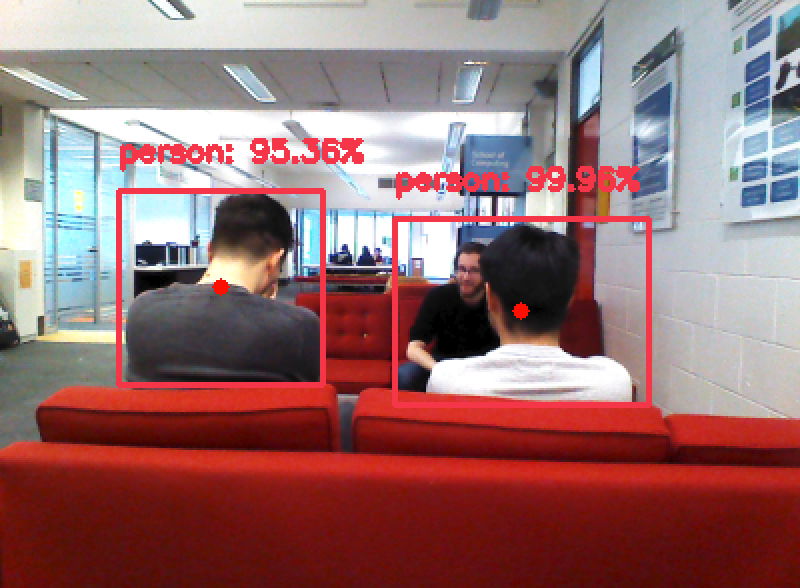
\includegraphics[width=.9\linewidth]{images/chapter6_occlusion_seated.png}
        \caption{Occlusion due to overlapping.}
	\end{subfigure}
    \begin{subfigure}{.5\textwidth}
        \centering
        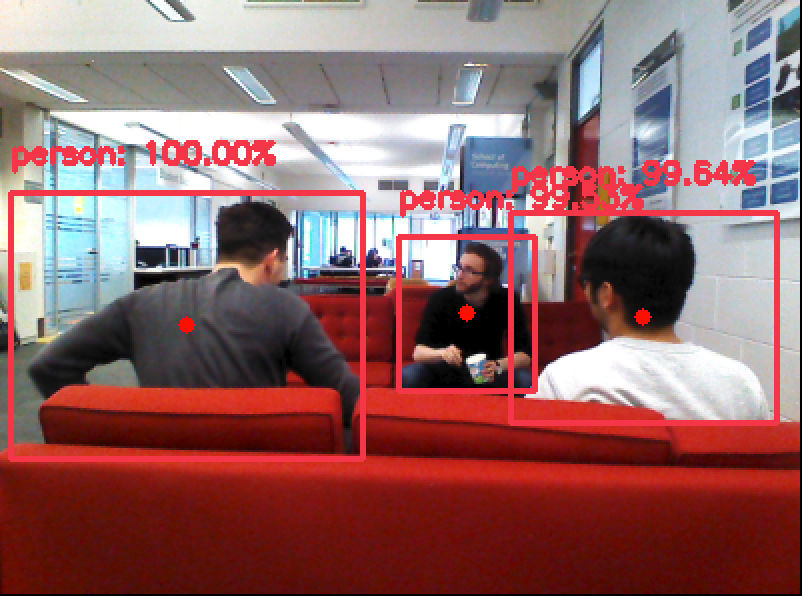
\includegraphics[width=.9\linewidth]{images/chapter6_occlusion_seated_good.png}
        \caption{Correct detection in occlusion.}
	\end{subfigure}
    \begin{subfigure}{.5\textwidth}
        \centering
        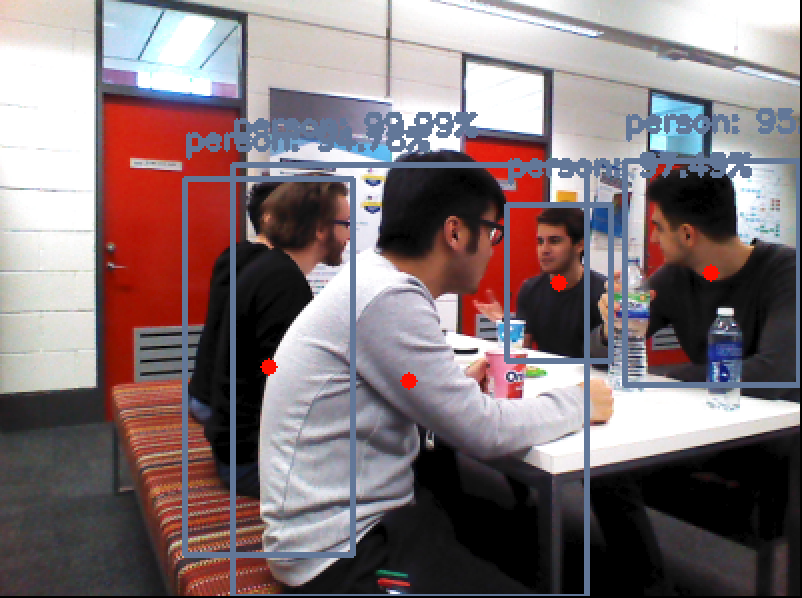
\includegraphics[width=.9\linewidth]{images/chapter6_occlusion_table_back.png}
        \caption{Seated occlusion.}
	\end{subfigure}
    \begin{subfigure}{.5\textwidth}
        \centering
        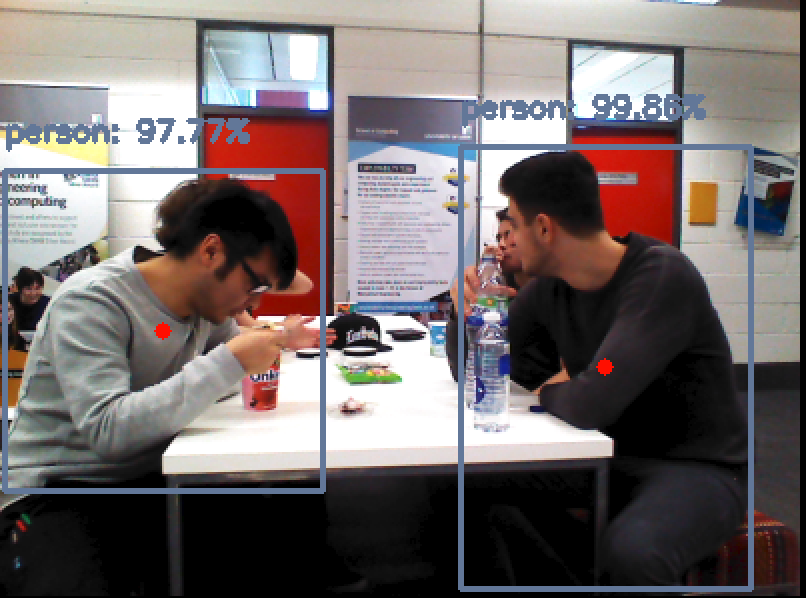
\includegraphics[width=.9\linewidth]{images/chapter6_occlusion_table_side.png}
        \caption{Sideway occlusion.}
	\end{subfigure}
\end{figure}

In Figure (a) the neural network fails at separating between the two subjects sitting to the right of the sofa, although the distinction is clearly visible. Figure (b) shows a good detection result when the occluding person moves to the right. Finally, we notice how in both (a) and (b) the two people sitting with their back towards the camera where detected even though only a part of their upper-back was showing, with an incredible 100\% confidence for one of the subjects in (b).

In Figure (c) the module is able to detect four out of the five participants, in a situation where three of these are either occluded by the table or other subjects. In (d) the same scenario as (c) is presented but from a side perspective. In this occasion only two people at the for-front are being detected as the remaining three subjects are completely or majority occluded by these.

\subsubsection{Final Conclusion}

The module can be considered to be highly reliable given its correctness in detecting people in all sorts of positions and variables, as well as its robustness against false positives instances as throughout the testing not once a non-person was detected as such.

\subsection{Pose Estimation}

To test the distance and 3D pose computations three different scenarios were carried out in the robotics lab. For each scenario the correct 3D pose of each individual was noted down along using the point cloud data in RVIZ. The measurement is then used as a comparison to the estimated 3D pose of the package. The red markers in the RVIZ images below show the estimated position while the violet ones the actual one.

\subsubsection{Scenario1}

\begin{figure}[H]
    \begin{subfigure}{.5\textwidth}
        \centering
        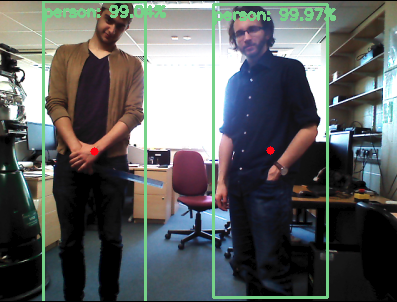
\includegraphics[width=\linewidth]{images/chapter6_scenario1.png}
        \caption{Scenario1 frame.}
        \label{2a}
	\end{subfigure}
    \begin{subfigure}{.5\textwidth}
        \centering
        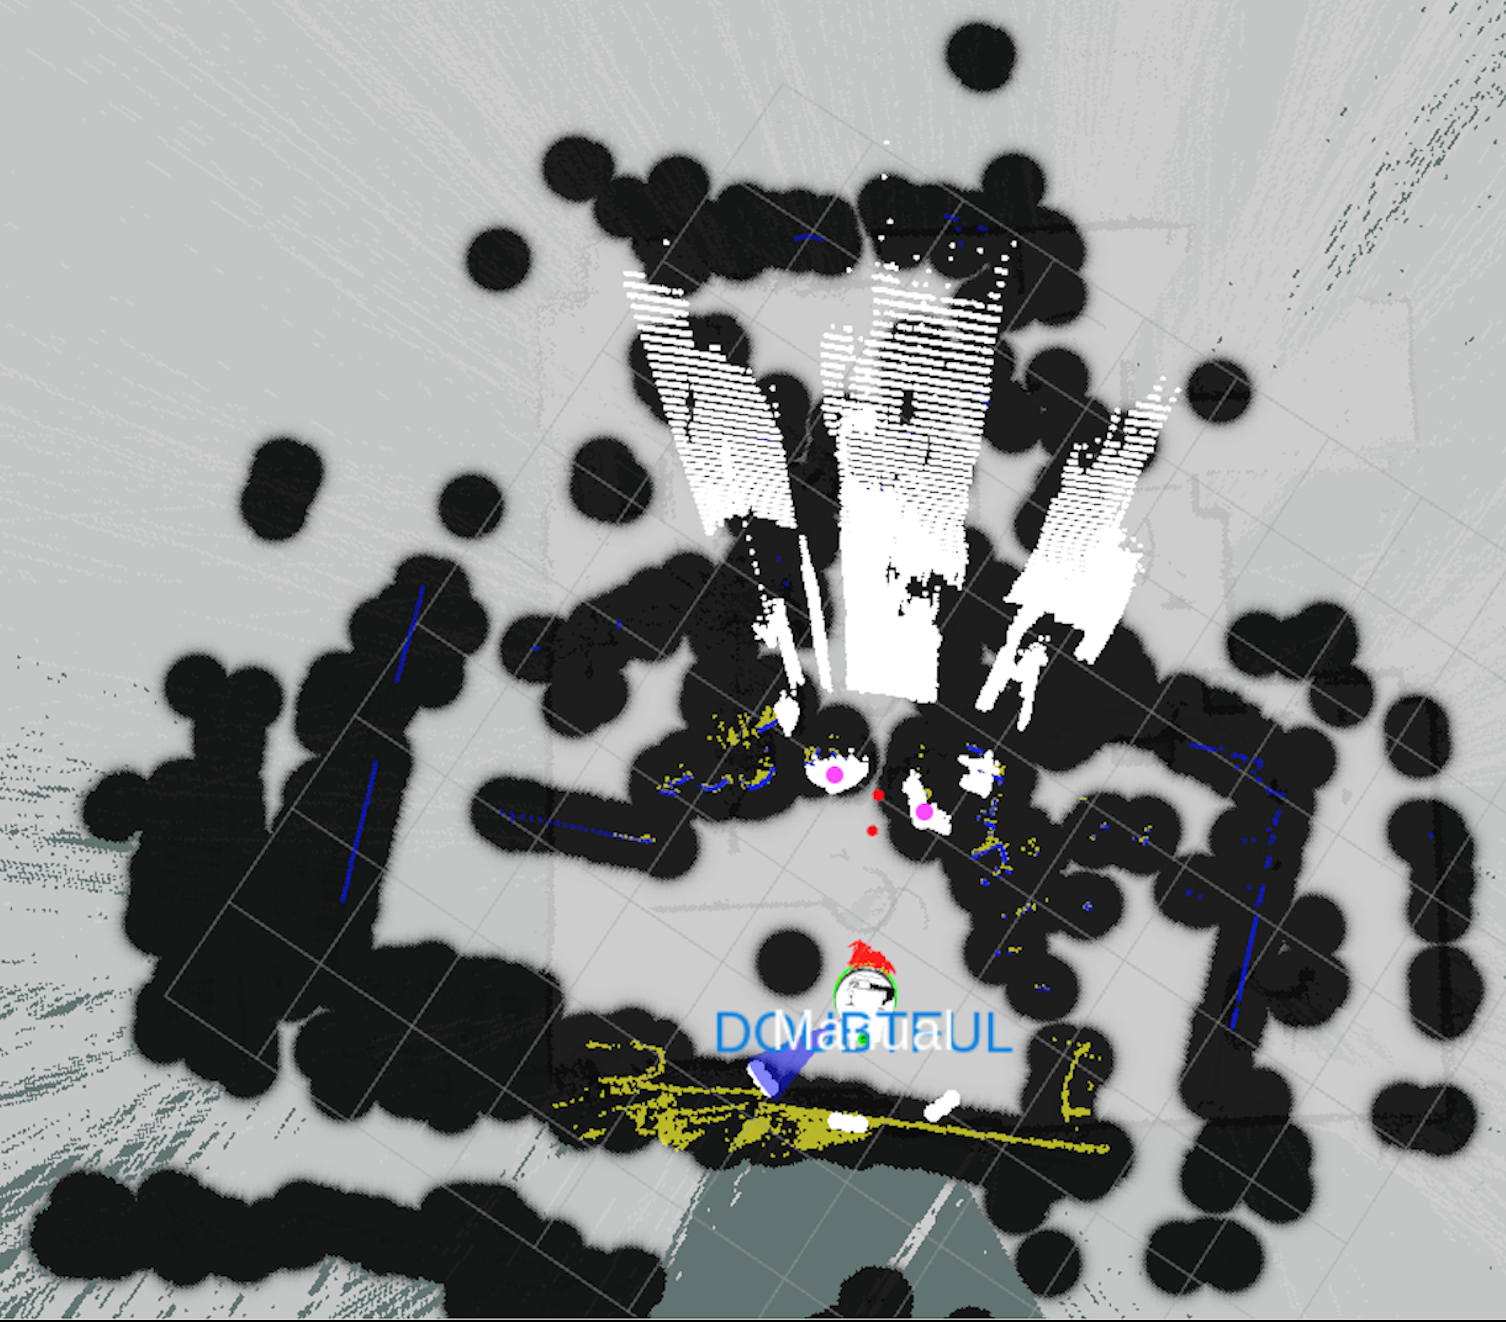
\includegraphics[width=\linewidth]{images/chapter6_rviz_extend.png}
        \caption{Scenario1 markers.}
        \label{2b}
	\end{subfigure}
\end{figure}

\begin{table}[H]
  \centering
  \begin{tabular}{ |p{4cm}|p{2cm}|p{2cm}|p{2cm}|  }
    \hline
    \multicolumn{4}{|c|}{Scenario1: 3D Pose Data} \\
    \hline
    & \textbf{X} & \textbf{Y} & \textbf{Z} \\
    \hline
    Real (Left) & 0.856 & 0.633 & 0.00293 \\
    Estimated (Left) & 0.738 & 0.519 & 0.00203 \\
    \hline
    Real (Right) & 0.0497 & 0.264 & 0.00149 \\
    Estimated (Right) & 0.0623 & 0.192 & 0.00475 \\
    \hline
  \end{tabular}
\end{table}



\subsubsection{Scenario2}

\begin{figure}[H]
    \begin{subfigure}{.5\textwidth}
        \centering
        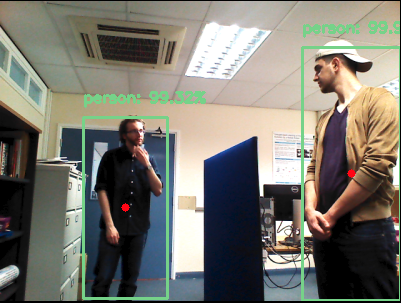
\includegraphics[width=8cm]{images/chapter6_scenario2.png}
        \caption{Scenario1 frame.}
        \label{2a}
	\end{subfigure}
    \begin{subfigure}{.5\textwidth}
        \centering
        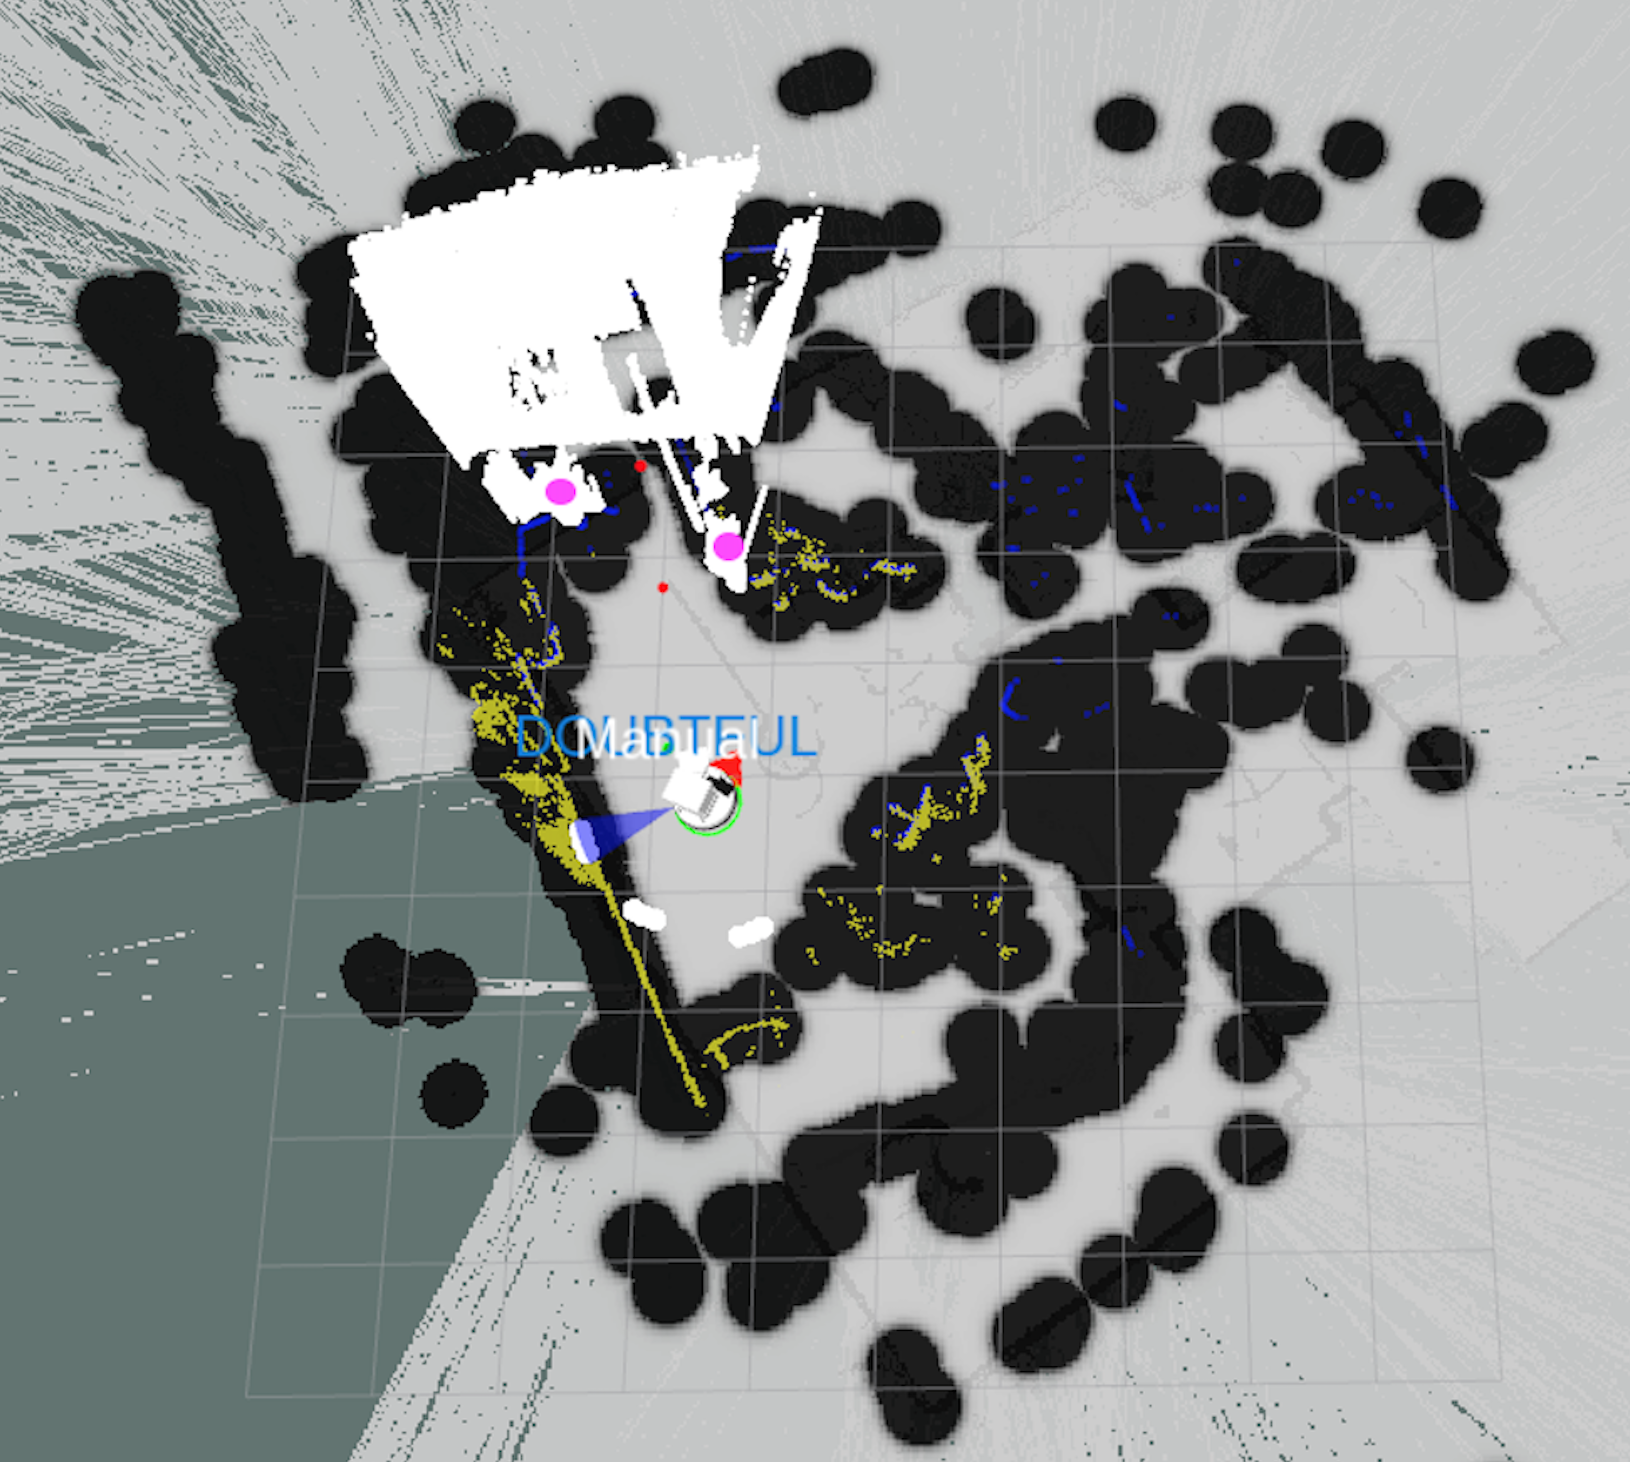
\includegraphics[width=.9\linewidth]{images/chapter6_rviz_extend2.png}
        \caption{Scenario1 markers.}
        \label{2b}
	\end{subfigure}
\end{figure}

\begin{table}[H]
  \centering
  \begin{tabular}{ |p{4cm}|p{2cm}|p{2cm}|p{2cm}|  }
    \hline
    \multicolumn{4}{|c|}{Scenario1: 3D Pose Data} \\
    \hline
    & \textbf{X} & \textbf{Y} & \textbf{Z} \\
    \hline
    Real (Left) & 2.17 & 2.61 & 0.00248 \\
    Estimated (Left) & 2.63 & 2.11 & 0.00357 \\
    \hline
    Real (Right) & 1.73 & 1.11 & 0.00547 \\
    Estimated (Right) & 1.4 & 1.67 & 0.00666 \\
    \hline
  \end{tabular}
\end{table}
\clearpage

\subsubsection{Scenario3}

\begin{figure}[H]
    \begin{subfigure}{.5\textwidth}
        \centering
        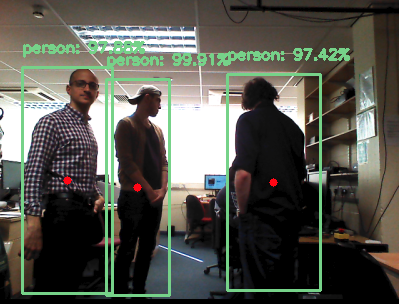
\includegraphics[width=8cm]{images/chapter6_scenario3.png}
        \caption{Scenario1 frame.}
        \label{2a}
	\end{subfigure}
    \begin{subfigure}{.5\textwidth}
        \centering
        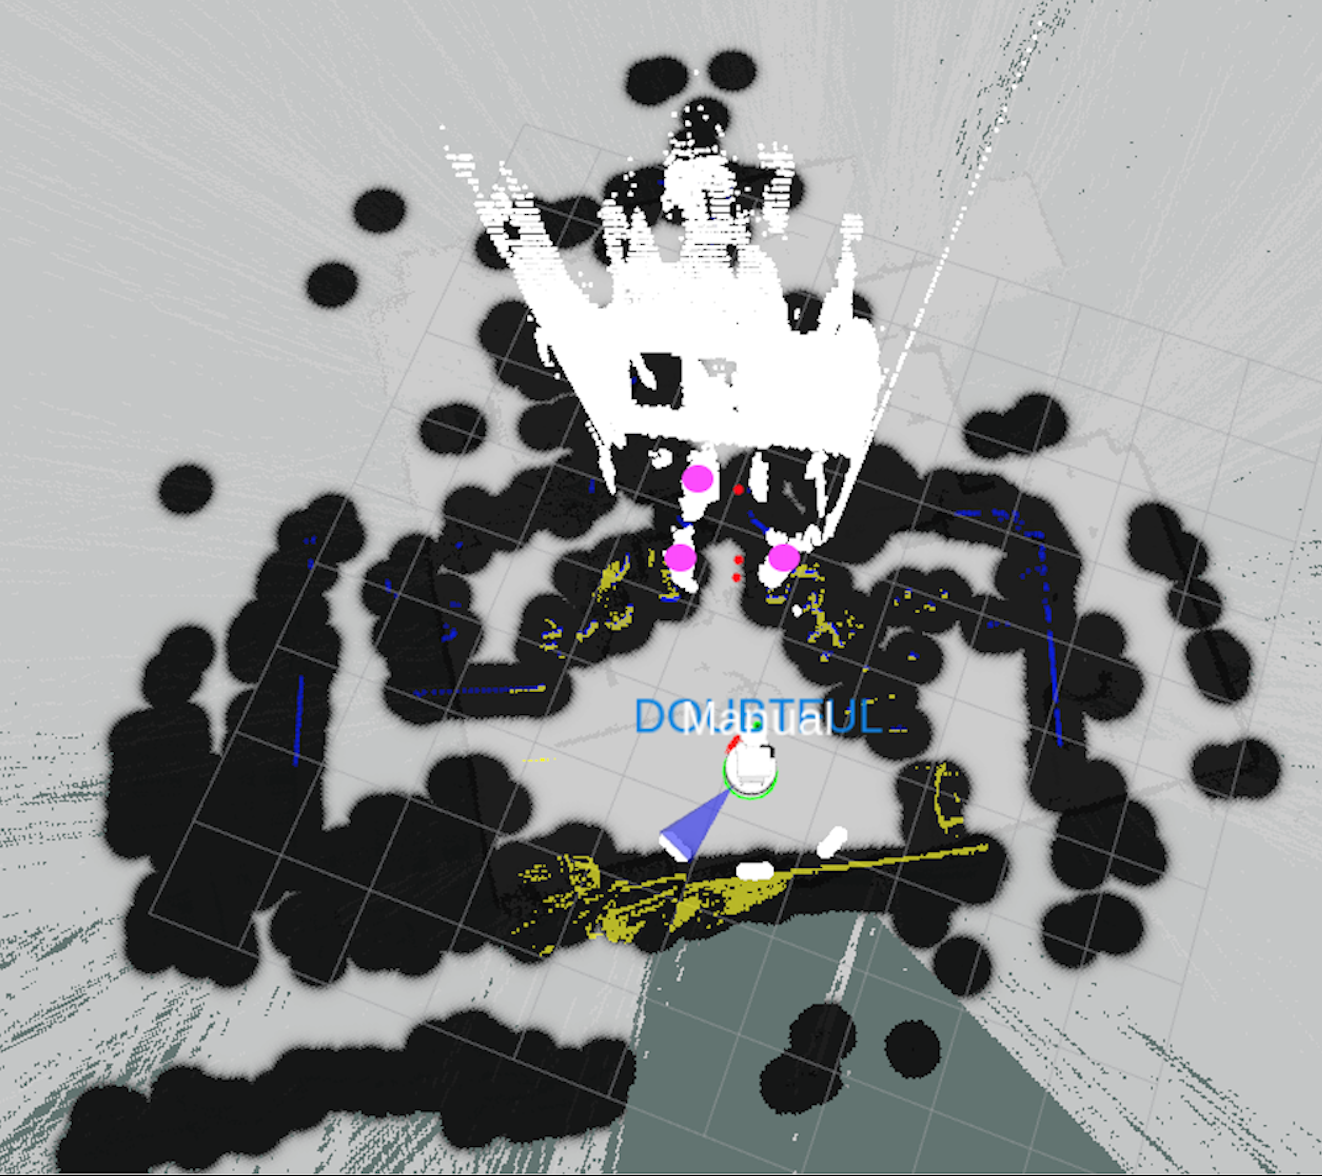
\includegraphics[width=.9\linewidth]{images/chapter6_extend3.png}
        \caption{Scenario1 markers.}
        \label{2b}
	\end{subfigure}
\end{figure}

\begin{table}[H]
  \centering
  \begin{tabular}{ |p{4cm}|p{2cm}|p{2cm}|p{2cm}|  }
    \hline
    \multicolumn{4}{|c|}{Scenario1: 3D Pose Data} \\
    \hline
    & \textbf{X} & \textbf{Y} & \textbf{Z} \\
    \hline
    Real (Left) & 1.33 & 0.0972 & 0.00441 \\
    Estimated (Left) & 1.21 & 0.124 & 0.00203 \\
    \hline
    Real (Centre) & 0.0497 & 0.264 & 0.00149 \\
    Estimated (Centre) & 0.283 & 0.344 & 0.00475 \\
    \hline
    Real(Right) & 0.0497 & 0.264 & 0.00149 \\
    Estimated(Right) & 0.283 & 0.344 & 0.00475 \\
    \hline
  \end{tabular}
\end{table}

  \chapter{Planning \& Project Management}
\label{chapter7}

In this chapter the planning and project management techniques used throughout the project in order to mitigate the inherent risk of the experimentation are discussed, with a focus on how the project was broke down into its phases, the source version control and other project management techniques.

The Gantt chart with the project's weekly breakdowns is available in Appendix D.

\section{Change of aim}

The nature of the project and its experimentation approach, the intermediate report feedback received by Dr. Mehmet Dogar, the project's assessor, were such that the original aim of the project was changed in agreement with Dr. Matteo Leonetti, the project's supervisor, so as not to incorporate the original human-robot behavioural aspect that should have seen the robot not only detect the human pose in the environment, but join these whenever there was on-going discussion. However, as the change happened at a relatively early development stage, and the previous background research done was still relative to the re-shaped project not much re-planning was necessary for the ultimate fulfillment of the task.

\section{Planning}

The project development followed an agile methodology, where four main phases were identified for a successful accomplishment.

The first phase consisted in developing the human detection piece which was the essential part of the project, as without a correct and precise recognition the remaining modules would serve nothing.

The second phase consisted in obtaining a correct and precise human-robot distance, which would allow a correct pose estimation later on.

The third phase was about finding the 3D world position of the detection in the world, where by world in this case is meant the map of the environment.

% The last and fourth module wasn't really development, but rather integration, as an off-the-shelf ROS package is used to give the user a possible esteem for detections outside of the 8 metres RGB-D range.

\section{GitHub}

The project's code is hosted entirely on GitHub as a public repository\footnote{ \url{https://github.com/itaouil/HARN}}, which makes it easily accessible to everyone who wants to contribute to it. Moreover, GitHub offers other project management techniques that have been used throughout the development and which are presented below.

\subsection{Branching}

Git branching was an important aspect of the development, in order to separate the different modules implementation and the major features within these. This enabled a safer experimenting process where already working features in the master branch were not affected by the on-going development of others. 

Moreover, the approach taken in the development consisted of merging to master after every feature completion, followed by the deletion of the latter's local and remote branch, hence, none of the development branches are still available on GitHub anymore, nonetheless, 4 branches have been used during the implementation part of the project for the following features:

\begin{itemize}
  \item Person detection module
  \item OpenCV conversion module
  \item RGB to Depth mapping
  \item Depth to 3D pose
\end{itemize}

\subsection{Milestones \& Issues}

GitHub issues have been used to keep track of uncompleted tasks as well as bugs encountered during the development phase. The standard GitHub issues labels have used to indicate the nature of the issue. Moreover, two Milestones have been identified, one for the marked presentation given before the easter break and one for the final submission deadline. Issues have been assigned accordingly to their respective Milestone.

\subsection{License}

As previously stated the ROS package developed will be made available to the open-source ROS community for them to use and improve. Hence the need to make the repository publicly available, thereby granting permission to everyone to use and modify the software, with the final aim of bringing further improvements to it.

Therefore, the repository, source code and all contents to it was licensed under the \textbf{General Public License v3.0}.

\subsection{Wiki}

Documentation is really important for open-source projects to document the correct installation process, dependencies, usage and possible encountered issues. Therefore a detailed wiki is kept within GitHub which would serve as a reference for future usage. 
  \chapter{Conclusions}
\label{chapter8}

\section{Limitations}

The end-result reached is certainly not perfect and has multiple limitations. One of these is the estimation latency brought by the RGB-depth synchronisation, which ultimately causes the chain to wait a couple of seconds before the next pose request is fired. This could limit the application usage of the package when high frame rates are required due to the dynamic environment.

Moreover, the ROS services used for the intra-module-communication, although offering an easy way to exchange messages between the various components, do limit the modularity of the package as all the modules would need to be run even if only the RGB detection is the only interest due to the client-server chained process.

Additionally, the conversion module does add to the project further computational costs, although these are contained. Nonetheless, solving the CvBridge compatibility issue with OpenCV 3.3.0 would allow the removal of an added step which could be easily integrated in the detection component.

Finally, both the detection and pose module have a degree of error. In fact, the detection process would certainly not be expected to perform as good in the detection of people as a human eye, and ultimately it could fail because of different environmental variables present or because it is something that the network has never seen before in the training data. Similarly, the 3D pose is most of the times incorrect up to a certain degree of error.

\section{Future Improvements}

To solve the latency issue only one options is really available. This consists in decreasing the publishing frequency of the raw RGB image such that it is synchronised with the raw depth-image stream more often. Increasing the publication stream of the depth-image is not an option as the depth-computation performed by the RGB-D sensor takes time.

The intra-module-communication limitation, differently from the latency issues, has an effective solution, which is to use just the publish-subscribe paradigm. Therefore getting rid of the synchronised chain process between the modules. Moreover, such an approach would allow the user to use only the desired module, although the pose component would still require the detection's publications.

Compiling from source the latest OpenCV release and resolving the issues with the already present static binding would make the conversion module redundant in its task, as the raw image conversion could be tackled using the updated CvBridge bindings directly in the detection module.

Bringing further improvements to the detection module would consist in potentially re-training the neural network with more data. Nonetheless, such an improvement is not really required given the already robust solution. However, to reduce the 3D error estimation a better calibration to the factory one can be carried out using available ROS packages, which could potentially improve the pixel projection and the 3D conversion result.

\section{Personal Reflection}

At the beginning of the academic year I didn't know much about Robotics nor Computer Vision and I ignored the fact the latter existed at all as a topic. Fast forward a couple of months into the year and I had the chance to discover some of the fundamental aspects behind both fields, through lectures and a group project where both aspects were put into practice. Towards the end of the module I knew that Robotics is what I wanted to pursue as a future career because of its challenges and the opportunity to work on so many different topics that intersects within it.

Hence the decision to carry out the following research project to further explore the field and advance in my personal knowledge. Throughout the project I learnt how to tackle a research task whose objectives are not precisely defined and how to implement abstract ideas read on papers in a constrained amount of time, increasing my organisational, analytical and problem solving skills.

I thoroughly enjoyed working on the project and I am happy to have created something useful for the open-source robotics community and for the University of Leeds RoboCup team, which I hope they will use to win many competitions in the future.

Moreover, thanks to this project I understood the importance that open-source projects have in such a field, and I am looking forward to contribute more to the open-source community in the future.






  \chapter{Conclusions}
\label{chapter9}

\section{TODO}

  % References
  \addcontentsline{toc}{chapter}{References}
  \bibliography{refs}. 

  % Appendices
  \begin{appendices}
\chapter{Legal, ethical, social and professional issues}

\textbf{Privacy Issues}

One of the burning ethical issues is surely the privacy of the data that such autonomous system can easily collect within their environment and ultimately process or store locally or even in the cloud. This project does not store any data, which in this case might be pictures of people in the room.

\textbf{Unemployment and Wealth redistribution}

Unemployment is another issue that sooner or later has to be tackled, as robots become more and more capable of doing predictable and unpredictable jobs there is a high risk of people loosing their jobs in different areas including care, construction and drivers. This project is not necessarily involved in any of these sectors, nonetheless, such a professional issues should be taken into consideration. 

Wealth redistribution is another pressing topic. How shall the income brought by these robots be managed, should a part of it be given back to the people that lost their jobs to the hands of these autonomous and efficient systems or not.

\textbf{Human Robot Interaction}

Robots, such as the one described in this project will become soon part of the environment we live in, not that we already don't live with robots (printers, smart-phones, Teslas, etc), but these intelligent systems will gain a certain human behavior in their movement, in their talk and in their ability to interact. This could possibly affect the way we understand interaction and change us in the worse. Just imagine a Robot which is able to change its talk cadence, movements and emotions depending on the person in front of it, wouldn't this affect us in the same way as well.

% There should only be one appendix in the intermediate report, for ethical issues.
\end{appendices}
\end{document}

